% Options for packages loaded elsewhere
\PassOptionsToPackage{unicode}{hyperref}
\PassOptionsToPackage{hyphens}{url}
\PassOptionsToPackage{dvipsnames,svgnames,x11names}{xcolor}
%
\documentclass[
  10pt,
]{article}
\usepackage{amsmath,amssymb}
\usepackage{iftex}
\ifPDFTeX
  \usepackage[T1]{fontenc}
  \usepackage[utf8]{inputenc}
  \usepackage{textcomp} % provide euro and other symbols
\else % if luatex or xetex
  \usepackage{unicode-math} % this also loads fontspec
  \defaultfontfeatures{Scale=MatchLowercase}
  \defaultfontfeatures[\rmfamily]{Ligatures=TeX,Scale=1}
\fi
\usepackage{lmodern}
\ifPDFTeX\else
  % xetex/luatex font selection
\fi
% Use upquote if available, for straight quotes in verbatim environments
\IfFileExists{upquote.sty}{\usepackage{upquote}}{}
\IfFileExists{microtype.sty}{% use microtype if available
  \usepackage[]{microtype}
  \UseMicrotypeSet[protrusion]{basicmath} % disable protrusion for tt fonts
}{}
\makeatletter
\@ifundefined{KOMAClassName}{% if non-KOMA class
  \IfFileExists{parskip.sty}{%
    \usepackage{parskip}
  }{% else
    \setlength{\parindent}{0pt}
    \setlength{\parskip}{6pt plus 2pt minus 1pt}}
}{% if KOMA class
  \KOMAoptions{parskip=half}}
\makeatother
\usepackage{xcolor}
\usepackage[left=2cm, right=2cm, top=2cm, bottom=3cm, footskip = .5cm]{geometry}
\usepackage{longtable,booktabs,array}
\usepackage{calc} % for calculating minipage widths
% Correct order of tables after \paragraph or \subparagraph
\usepackage{etoolbox}
\makeatletter
\patchcmd\longtable{\par}{\if@noskipsec\mbox{}\fi\par}{}{}
\makeatother
% Allow footnotes in longtable head/foot
\IfFileExists{footnotehyper.sty}{\usepackage{footnotehyper}}{\usepackage{footnote}}
\makesavenoteenv{longtable}
\usepackage{graphicx}
\makeatletter
\def\maxwidth{\ifdim\Gin@nat@width>\linewidth\linewidth\else\Gin@nat@width\fi}
\def\maxheight{\ifdim\Gin@nat@height>\textheight\textheight\else\Gin@nat@height\fi}
\makeatother
% Scale images if necessary, so that they will not overflow the page
% margins by default, and it is still possible to overwrite the defaults
% using explicit options in \includegraphics[width, height, ...]{}
\setkeys{Gin}{width=\maxwidth,height=\maxheight,keepaspectratio}
% Set default figure placement to htbp
\makeatletter
\def\fps@figure{htbp}
\makeatother
\setlength{\emergencystretch}{3em} % prevent overfull lines
\providecommand{\tightlist}{%
  \setlength{\itemsep}{0pt}\setlength{\parskip}{0pt}}
\setcounter{secnumdepth}{-\maxdimen} % remove section numbering
% Set up the fonts
\usepackage[urw-palatino]{mathdesign}
\usepackage[T1]{fontenc}

% Add accessibility support from http://www.richschwinn.com/accessibility
\RequirePackage{accsupp}
\RequirePackage{pdfcomment}
\newcommand{\AccTool}[2]{\BeginAccSupp{method=pdfstringdef,unicode,Alt={{#1}}}\pdftooltip{{#2}}{{#1}}\EndAccSupp{}}

% Set the language for 508
\hypersetup{
  pdftitle = {title},
  pdflang = en-US}


% Set up the headers and footers
\usepackage{graphicx}
\usepackage{fancyhdr}
\usepackage{ifthen}
%\usepackage{everypage-1x}
\usepackage{float}
%\usepackage{subfig}
%\usepackage{subcaption}

% Avoid struggling over figure and table float in Rmarkdown
\let\origfigure\figure
\let\endorigfigure\endfigure
\renewenvironment{figure}[1][2] {
    \expandafter\origfigure\expandafter[H]
} {
    \endorigfigure
}

\let\origtable\table
\let\endorigtable\endtable
\renewenvironment{table}[1][2] {
    \expandafter\origtable\expandafter[H]
} {
    \endorigtable
}

% First page has the large title and NOAA logo
\pagestyle{fancy}
\fancyhf{}
\setlength\headheight{40pt}
\fancyheadoffset[L]{0.5cm}
\cfoot{\thepage}

\fancyheadinit{%
   \ifthenelse{\value{page}=5}%
      {\fancyhead[R]{
\includegraphics[width=40pt]{images/NOAA_logo.png} \\ \textsf{\emph{February 9, 2023}}}
       \fancyhead[L]{\textsf{\LARGE DRAFT State of the Ecosystem 2024: New England}}
      }%
      {\fancyhead[R]{}
       \fancyhead[L]{\textsf{\emph{DRAFT State of the Ecosystem 2024: New England}}}
      }
}



\renewcommand{\headrulewidth}{0.4pt}
\renewcommand{\footrulewidth}{0pt}

% Make caption fonts a bit smaller
\usepackage[font={small}]{caption}


% Change section labels to san serif
\usepackage{sectsty}
\allsectionsfont{\normalfont\sffamily\bfseries}
\usepackage{multirow}
\usepackage{multicol}
\usepackage{colortbl}
\usepackage{hhline}
\newlength\Oldarrayrulewidth
\newlength\Oldtabcolsep
\usepackage{longtable}
\usepackage{array}
\usepackage{hyperref}
\usepackage{float}
\usepackage{wrapfig}
\ifLuaTeX
  \usepackage{selnolig}  % disable illegal ligatures
\fi
\IfFileExists{bookmark.sty}{\usepackage{bookmark}}{\usepackage{hyperref}}
\IfFileExists{xurl.sty}{\usepackage{xurl}}{} % add URL line breaks if available
\urlstyle{same}
\hypersetup{
  colorlinks=true,
  linkcolor={Maroon},
  filecolor={Maroon},
  citecolor={Blue},
  urlcolor={blue},
  pdfcreator={LaTeX via pandoc}}

\author{}
\date{\vspace{-2.5em}}

\begin{document}

\setcounter{page}{5}
\thispagestyle{fancy}

\hypertarget{introduction}{%
\section{Introduction}\label{introduction}}

\hypertarget{about-this-report}{%
\subsection{About This Report}\label{about-this-report}}

This report is for the New England Fishery Management Council (NEFMC). The purpose of this report is to synthesize ecosystem information to allow the NEFMC to better meet fishery management objectives. The major messages of the report are summarized on pages 1, 2, and 3, and synthesis themes are illustrated on page 4. Information in this report is organized into two sections; \protect\hyperlink{performance-relative-to-fishery-management-objectives}{performance measured against ecosystem-level management objectives} (Table \ref{tab:management-objectives}), and potential \protect\hyperlink{risks-to-meeting-fishery-management-objectives}{risks to meeting fishery management objectives} (\protect\hyperlink{climate-and-ecosystem-productivity}{climate change} and \protect\hyperlink{other-ocean-uses-offshore-wind}{other ocean uses}).

\hypertarget{report-structure}{%
\subsection{Report structure}\label{report-structure}}

The two main sections contain subsections for each management objective or potential risk. Within each subsection, we first review indicator trends, and the status of the most recent data year relative to a threshold (if available) or relative to the long-term average. Second, we synthesize results of other indicators and information to outline potential implications for management (i.e., connecting indicator(s) status to management and why an indicator(s) is important). For example, if there are multiple drivers related to an indicator trend, which drivers may be more or less supported by current information, and which, if any, can be affected by management action(s)? Similarly, which risk indicators warrant continued monitoring to evaluate whether regime shifts or ecosystem reorganization are likely? We emphasize that these implications are intended to represent testable hypotheses at present, rather than ``answers,'' because the science behind these indicators and syntheses continues to develop.

A glossary of terms\footnote{\url{https://noaa-edab.github.io/tech-doc/glossary.html}}, detailed technical methods documentation\footnote{\url{https://NOAA-EDAB.github.io/tech-doc}} and indicator data\footnote{\url{https://github.com/NOAA-EDAB/ecodata}}, and detailed indicator descriptions\footnote{\url{https://noaa-edab.github.io/catalog/index.html}} are available online. The details of standard figure formatting (Fig. \ref{fig:docformat}a), categorization of fish and invertebrate species into feeding groups (Table \ref{tab:species-groupings}), and definitions of ecological production units (EPUs, including Georges Bank, GB, and the Gulf of Maine, GOM; Fig. \ref{fig:docformat}b) are provided at the end of the document.

\global\setlength{\Oldarrayrulewidth}{\arrayrulewidth}

\global\setlength{\Oldtabcolsep}{\tabcolsep}

\setlength{\tabcolsep}{0pt}

\renewcommand*{\arraystretch}{1}



\providecommand{\ascline}[3]{\noalign{\global\arrayrulewidth #1}\arrayrulecolor[HTML]{#2}\cline{#3}}

\begin{longtable}[c]{|p{1.42in}|p{4.09in}}

\caption{Example\ ecosystem-scale\ fishery\ management\ objectives\ for\ the\ New\ England\ region}\label{tab:management-objectives}\\

\ascline{1.5pt}{666666}{1-2}

\multicolumn{1}{>{\raggedright}m{\dimexpr 1.42in+0\tabcolsep}}{\textcolor[HTML]{000000}{\fontsize{9}{9}\selectfont{Objective\ categories}}} & \multicolumn{1}{>{\raggedright}m{\dimexpr 4.09in+0\tabcolsep}}{\textcolor[HTML]{000000}{\fontsize{9}{9}\selectfont{Indicators\ reported}}} \\

\ascline{1.5pt}{666666}{1-2}\endfirsthead \caption[]{Example\ ecosystem-scale\ fishery\ management\ objectives\ for\ the\ New\ England\ region}\label{tab:management-objectives}\\

\ascline{1.5pt}{666666}{1-2}

\multicolumn{1}{>{\raggedright}m{\dimexpr 1.42in+0\tabcolsep}}{\textcolor[HTML]{000000}{\fontsize{9}{9}\selectfont{Objective\ categories}}} & \multicolumn{1}{>{\raggedright}m{\dimexpr 4.09in+0\tabcolsep}}{\textcolor[HTML]{000000}{\fontsize{9}{9}\selectfont{Indicators\ reported}}} \\

\ascline{1.5pt}{666666}{1-2}\endhead



\multicolumn{2}{>{\raggedright}m{\dimexpr 5.51in+2\tabcolsep}}{\textcolor[HTML]{000000}{\fontsize{9}{9}\selectfont{\textbf{Provisioning\ and\ Cultural\ Services}}}} \\





\multicolumn{1}{>{\raggedright}m{\dimexpr 1.42in+0\tabcolsep}}{\textcolor[HTML]{000000}{\fontsize{9}{9}\selectfont{Seafood\ Production}}} & \multicolumn{1}{>{\raggedright}m{\dimexpr 4.09in+0\tabcolsep}}{\textcolor[HTML]{000000}{\fontsize{9}{9}\selectfont{Landings;\ commercial\ total\ and\ by\ feeding\ guild;\ recreational\ harvest}}} \\





\multicolumn{1}{>{\raggedright}m{\dimexpr 1.42in+0\tabcolsep}}{\textcolor[HTML]{000000}{\fontsize{9}{9}\selectfont{Profits}}} & \multicolumn{1}{>{\raggedright}m{\dimexpr 4.09in+0\tabcolsep}}{\textcolor[HTML]{000000}{\fontsize{9}{9}\selectfont{Revenue\ decomposed\ to\ price\ and\ volume}}} \\





\multicolumn{1}{>{\raggedright}m{\dimexpr 1.42in+0\tabcolsep}}{\textcolor[HTML]{000000}{\fontsize{9}{9}\selectfont{Recreation}}} & \multicolumn{1}{>{\raggedright}m{\dimexpr 4.09in+0\tabcolsep}}{\textcolor[HTML]{000000}{\fontsize{9}{9}\selectfont{Days\ fished;\ recreational\ fleet\ diversity}}} \\





\multicolumn{1}{>{\raggedright}m{\dimexpr 1.42in+0\tabcolsep}}{\textcolor[HTML]{000000}{\fontsize{9}{9}\selectfont{Stability}}} & \multicolumn{1}{>{\raggedright}m{\dimexpr 4.09in+0\tabcolsep}}{\textcolor[HTML]{000000}{\fontsize{9}{9}\selectfont{Diversity\ indices\ (fishery\ and\ ecosystem)}}} \\





\multicolumn{1}{>{\raggedright}m{\dimexpr 1.42in+0\tabcolsep}}{\textcolor[HTML]{000000}{\fontsize{9}{9}\selectfont{Social\ \&\ Cultural}}} & \multicolumn{1}{>{\raggedright}m{\dimexpr 4.09in+0\tabcolsep}}{\textcolor[HTML]{000000}{\fontsize{9}{9}\selectfont{Community\ engagement/reliance\ status}}} \\





\multicolumn{1}{>{\raggedright}m{\dimexpr 1.42in+0\tabcolsep}}{\textcolor[HTML]{000000}{\fontsize{9}{9}\selectfont{Protected\ Species}}} & \multicolumn{1}{>{\raggedright}m{\dimexpr 4.09in+0\tabcolsep}}{\textcolor[HTML]{000000}{\fontsize{9}{9}\selectfont{Bycatch;\ population\ (adult\ and\ juvenile)\ numbers,\ mortalities}}} \\





\multicolumn{2}{>{\raggedright}m{\dimexpr 5.51in+2\tabcolsep}}{\textcolor[HTML]{000000}{\fontsize{9}{9}\selectfont{\textbf{Supporting\ and\ Regulating\ Services}}}} \\





\multicolumn{1}{>{\raggedright}m{\dimexpr 1.42in+0\tabcolsep}}{\textcolor[HTML]{000000}{\fontsize{9}{9}\selectfont{Biomass}}} & \multicolumn{1}{>{\raggedright}m{\dimexpr 4.09in+0\tabcolsep}}{\textcolor[HTML]{000000}{\fontsize{9}{9}\selectfont{Biomass\ or\ abundance\ by\ feeding\ guild\ from\ surveys}}} \\





\multicolumn{1}{>{\raggedright}m{\dimexpr 1.42in+0\tabcolsep}}{\textcolor[HTML]{000000}{\fontsize{9}{9}\selectfont{Productivity}}} & \multicolumn{1}{>{\raggedright}m{\dimexpr 4.09in+0\tabcolsep}}{\textcolor[HTML]{000000}{\fontsize{9}{9}\selectfont{Condition\ and\ recruitment\ of\ managed\ species,\ Primary\ productivity}}} \\





\multicolumn{1}{>{\raggedright}m{\dimexpr 1.42in+0\tabcolsep}}{\textcolor[HTML]{000000}{\fontsize{9}{9}\selectfont{Trophic\ structure}}} & \multicolumn{1}{>{\raggedright}m{\dimexpr 4.09in+0\tabcolsep}}{\textcolor[HTML]{000000}{\fontsize{9}{9}\selectfont{Relative\ biomass\ of\ feeding\ guilds,\ Zooplankton}}} \\





\multicolumn{1}{>{\raggedright}m{\dimexpr 1.42in+0\tabcolsep}}{\textcolor[HTML]{000000}{\fontsize{9}{9}\selectfont{Habitat}}} & \multicolumn{1}{>{\raggedright}m{\dimexpr 4.09in+0\tabcolsep}}{\textcolor[HTML]{000000}{\fontsize{9}{9}\selectfont{Estuarine\ and\ offshore\ habitat\ conditions}}} \\

\ascline{1.5pt}{666666}{1-2}



\end{longtable}



\arrayrulecolor[HTML]{000000}

\global\setlength{\arrayrulewidth}{\Oldarrayrulewidth}

\global\setlength{\tabcolsep}{\Oldtabcolsep}

\renewcommand*{\arraystretch}{1}

\hypertarget{performance-relative-to-fishery-management-objectives}{%
\section{Performance relative to fishery management objectives}\label{performance-relative-to-fishery-management-objectives}}

In this section, we examine indicators related to broad, ecosystem-level fishery management objectives. We also provide hypotheses on the implications of these trends---\emph{why} we are seeing them, what's driving them, and potential or observed regime shifts or changes in ecosystem structure. Identifying multiple drivers, regime shifts, and potential changes to ecosystem structure, as well as identifying the most vulnerable resources, can help managers determine whether anything differently needs to be done to meet objectives and how to prioritize upcoming issues/risks.

\hypertarget{seafood-production}{%
\subsection{Seafood Production}\label{seafood-production}}

\hypertarget{indicator-landings-commercial-and-recreational}{%
\subsubsection{Indicator: Landings; commercial and recreational}\label{indicator-landings-commercial-and-recreational}}

This year, we present updated \href{https://noaa-edab.github.io/catalog/commercial-landings-and-revenue.html}{indicators} for total commercial landings, U.S. seafood landings, and Council-managed U.S. seafood landings . Total commercial landings (black) within New England show no long-term trends (Fig. \ref{fig:total-landings}). We treat the last three years of total landings as preliminary, given that the Canadian landings within each EPU have yet to be updated by NAFO. There exist long term downward trends in commercial seafood landings for the Gulf of Maine, but over the last decade landings appear to be relatively stable. In addition, NEFMC managed seafood production on Georges Bank now presents a long term decreasing trend.

\begin{figure}

{\centering \includegraphics{SOE-NEFMC_files/figure-latex/total-landings-1} 

}

\caption{Total commercial landings (black), total U.S. seafood landings (blue), and New England managed U.S. seafood landings (red) for Georges Bank and the Gulf of Maine. Open circles represent years that are lacking NAFO (foreign) data. mt = metric tons}\label{fig:total-landings}
\end{figure}

Commercial landings by guild include all species and all uses, and are reported as total for the guild and the NEFMC managed species within the \href{https://noaa-edab.github.io/catalog/feeding-guilds-by-management-bodies.html}{guild}. As reported in previous years, downward trends persist for a number of guilds in both regions. A significant upward trend is present for benthivores (GOM), attributable to an increase in American lobster, and benthos (GB), attributable to clams and scallops (Fig. \ref{fig:comm-landings}). Landings of planktivores on Georges Bank are presenting mixed trends between total and managed species, both categories are near historic lows.

\begin{figure}

{\centering \includegraphics{SOE-NEFMC_files/figure-latex/comm-landings-1} 

}

\caption{Total commercial landings (black) and NEFMC managed U.S seafood landings (red) by feeding guild for the Gulf of Maine.}\label{fig:comm-landings}
\end{figure}

Overall, \href{https://noaa-edab.github.io/catalog/recreational-fishing-indicators.html}{recreational harvest} (retained fish presumed to be eaten) have also declined in New England (Fig. ). Although, harvest has rebounded somewhat from the historical low level in 2020. Recreational \href{https://noaa-edab.github.io/catalog/highly-migratory-species-landings.html}{shark landings} of pelagic and prohibited sharks have declined since 2018 (Fig \ref{fig:rec-landings}), likely influenced by regulatory changes implemented in 2018 intended to rebuild shortfin mako stocks.

\begin{figure}

{\centering \includegraphics{SOE-NEFMC_files/figure-latex/rec-landings-1} 

}

\caption{Total recreational seafood harvest (millions of pounds) in the New England region.}\label{fig:rec-landings}
\end{figure}
\begin{figure}

{\centering \includegraphics{SOE-NEFMC_files/figure-latex/rec-hms-1} 

}

\caption{Recreational shark landings from Large Pelagics Survey.}\label{fig:rec-hms}
\end{figure}

\href{https://noaa-edab.github.io/catalog/aquaculture-production.html}{Aquaculture production} is not yet included in total seafood landings.

\hypertarget{implications}{%
\subsubsection{Implications}\label{implications}}

Declining commercial seafood and recreational landings are driven by many interacting factors, including combinations of ecological and stock production, management actions, market conditions, and environmental changes. While we cannot evaluate all possible drivers at present, here we evaluate the extent to which stock status and changes in system biomass play a role.

\hypertarget{stock-status}{%
\paragraph{Stock Status}\label{stock-status}}

Single species \href{https://noaa-edab.github.io/catalog/stock-status.html}{management objectives} (1. maintaining biomass above minimum thresholds and 2. maintaining fishing mortality below overfishing limits) are not being met for some NEFMC managed species. Thirteen stocks are currently estimated to be below B\textbackslash textsubscript(MSY), while status relative to B\textbackslash textsubscript(MSY) could not be assessed for 13 additional stocks (Fig.\ref{fig:stock-status}). Therefore, stock status and associated management constraints are likely contributing to decreased landings. To better address the role of management in future reports, we could examine how the total allowable catch (TAC) and the percentage of the TAC taken for each species has changed through time.

\begin{figure}

{\centering \includegraphics{SOE-NEFMC_files/figure-latex/stock-status-1} 

}

\caption{Summary of single species status for NEFMC and jointly federally managed stocks (goosefish and spiny dogfish).  The dotted vertical line at one is the target biomass reference point of B.  The dashed lines are the management thresholds of B (vertical) or F (horizontal). Colors denote stocks with B/B\textsubscript{MSY} < 0.5 or F/F\textsubscript{MSY} (orange), stocks 0.5<B/B\textsubscript{MSY}<1 (blue), and stocks B/B\textsubscript{MSY}>1 (green).}\label{fig:stock-status}
\end{figure}

\hypertarget{system-biomass}{%
\paragraph{System Biomass}\label{system-biomass}}

\href{https://noaa-edab.github.io/catalog/aggregate-survey-biomass.html}{Aggregate biomass} trends derived from scientific resource surveys have been stable to increasing in both regions (Fig. \ref{fig:nefsc-biomass-gb} \& Fig. \ref{fig:nefsc-biomass-gom}). The benthivores group spiked during the last decade, due to a large haddock recruitment, but appears to be returning to average levels. Planktivore biomass on GB conitues to rise with the highest fall biomass observed since 1968. There are also increasing trends in piscivores, and planktivores in at least one season in both regions, and benthos on Georges Bank in both seasons. The New Hampshire/Maine state survey does not show these trends while the Massachusetts state survey shows the increasing trend in benthivores in the spring and planktivores in the fall but a decrease in piscivores in the spring and benthos in both seasons (Fig. \ref{fig:mass-biomass}). While managed species comprise varying proportions of aggregate biomass, trends in landings are not mirroring shifts in the overall trophic structure of survey-sampled fish and invertebrates. Therefore, major shifts in feeding guilds or ecosystem trophic structure are unlikely to be driving the decline in landings.

\begin{figure}

{\centering \includegraphics{SOE-NEFMC_files/figure-latex/nefsc-biomass-gb-1} 

}

\caption{Spring (left) and fall (right) surveyed biomass on Georges Bank. The shaded area around each annual mean represents 2 standard deviations from the mean.}\label{fig:nefsc-biomass-gb}
\end{figure}

\begin{figure}

{\centering \includegraphics{SOE-NEFMC_files/figure-latex/nefsc-biomass-gom-1} 

}

\caption{Spring (left) and fall (right) surveyed biomass in the Gulf of Maine. The shaded area around each annual mean represents 2 standard deviations from the mean.}\label{fig:nefsc-biomass-gom}
\end{figure}

\hypertarget{effect-on-seafood-production}{%
\paragraph{Effect on Seafood Production}\label{effect-on-seafood-production}}

With the poor or unknown stock status of many managed species, the decline in commercial seafood landings in the Gulf of Maine most likely reflects lower catch quotas implemented to rebuild overfished stocks, as well as market dynamics.

The decline in recreational seafood harvest stems from multiple drivers. Some of the decline, such as for recreational shark landings, continues to be driven by tightening regulations. However, changes in demographics and preferences over recreational activities likely play a role in non-HMS (Highly Migratory Species) declines in recreational harvest, with current harvests well below the time series average.

\begin{figure}

{\centering \includegraphics{SOE-NEFMC_files/figure-latex/mass-biomass-1} 

}

\caption{Spring (left) and fall (right) surveyed biomass from the state of Massachusetts inshore survey. The shaded area around each annual mean represents 2 standard deviations from the mean.}\label{fig:mass-biomass}
\end{figure}

Other environmental changes require monitoring as they may become important drivers of future landings:

\begin{itemize}
\tightlist
\item
  Climate is trending into uncharted territory. Globally, 2023 wasthe warmest year on record\footnote{\url{https://noaa-edab.github.io/catalog/observation-synthesis.html}} (see \protect\hyperlink{climate-and-ecosystem-productivity}{Climate Risks section}).
\item
  Stocks are shifting their distribution, moving towards the northeast and into deeper waters throughout the Northeast US Large Marine Ecosystem (Fig. \ref{fig:species-dist}).
\item
  Ecosystem composition and production changes have been observed (see \protect\hyperlink{stability}{Stability section}).
\item
  Some fishing communities are affected by environmental justice vulnerabilities (see \protect\hyperlink{social-vulnerability}{Environmental Justice and Social Vulnerability section}).
\end{itemize}

\newpage

\hypertarget{commercial-profits}{%
\subsection{Commercial Profits}\label{commercial-profits}}

\hypertarget{indicators-revenue-a-proxy-for-profits}{%
\subsubsection{Indicators: revenue (a proxy for profits)}\label{indicators-revenue-a-proxy-for-profits}}

\href{https://noaa-edab.github.io/catalog/commercial-landings-and-revenue.html}{Commercial revenue} in the region has been mostly positive with total commercial revenues from all species above the long-term mean for both the GB and GOM regions in 2022 (Fig. \ref{fig:comm-revenue}). However, revenue from NEFMC managed species shows a long-term downward trend in the GOM. GB continues to exhibit a cyclical nature with regards to revenue, largely driven by rotational management of Atlantic sea scallops.

\begin{figure}

{\centering \includegraphics{SOE-NEFMC_files/figure-latex/comm-revenue-1} 

}

\caption{Revenue through 2022 for the New England region: total (black) and from NEFMC managed species (red).}\label{fig:comm-revenue}
\end{figure}

Revenue earned by harvesting resources is a function of both the quantity landed of each species and the prices paid for landings. Beyond monitoring yearly changes in revenue, it is even more valuable to determine what drives these changes: harvest levels, the mix of species landed, price changes, or a combination of these. The {[}Bennet Indicator{]} (\url{https://noaa-edab.github.io/catalog/bennet-indicator.html}) decomposes revenue change into two parts, one driven by changing quantities (volumes), and a second driven by changing prices. All changes are in relation to a base year (1982).

In the GB region, revenues have been consistently lower than the 1982 baseline throughout the series. The changes in total revenue in GB was primarily driven by volumes prior to 2010, and then by prices (Fig.\ref{fig:bennet}). In the GOM, revenues have been above the 1982 baseline in all but four years, largely due to changing prices in most years. Breaking down the revenue by guild , for GB, both the volume and price trend have been largely driven by benthos (quahogs and surfclams). In the GOM region, increased prices for benthivores drove the year-over year increases in overall prices. Benthivores also had a large influence on the overall volume indicator in the GOM.

\begin{figure}

{\centering \includegraphics{SOE-NEFMC_files/figure-latex/bennet-1} 

}

\caption{Revenue change from the 1982 baseline in 2022 dollars (black), price, and volume for commercial landings from Georges Bank (GB: left) and the Gulf of Maine (GOM: right)}\label{fig:bennet}
\end{figure}
\begin{figure}

{\centering \includegraphics{SOE-NEFMC_files/figure-latex/bennet-all-1} 

}

\caption{Revenue change from the long-term mean in 2022 dollars (black), price, and volume for commercial landings from Georges Bank (GB: top panels) and the Gulf of Maine (GOM: bottom panels)}\label{fig:bennet-all}
\end{figure}

\hypertarget{implications-1}{%
\subsubsection{Implications}\label{implications-1}}

The continued dependence on lobster in the GOM and sea scallops on GB is affected by multiple drivers including resource availability and market conditions. As both species are sensitive to ocean warming and acidification, it is important to monitor these and other climate drivers.

\hypertarget{recreational-opportunities}{%
\subsection{Recreational Opportunities}\label{recreational-opportunities}}

\hypertarget{indicators-angler-trips-fleet-diversity}{%
\subsubsection{Indicators: Angler trips, fleet diversity}\label{indicators-angler-trips-fleet-diversity}}

\href{https://noaa-edab.github.io/catalog/recreational-fishing-indicators.html}{Recreational effort} (angler trips) increased during 1982-2010, but has since declined to the long-term average (Fig. \ref{fig:rec-op}). Recreational fleets are defined as private vessels, shore-based fishing, or party-charter vessels. Recreational fleet diversity, or the relative importance of each fleet type, has remained relatively stable over the latter half of the time series (Fig. \ref{fig:rec-div}).

\begin{figure}

{\centering \includegraphics{SOE-NEFMC_files/figure-latex/rec-op-1} 

}

\caption{Recreational effort in New England.}\label{fig:rec-op}
\end{figure}
\begin{figure}

{\centering \includegraphics{SOE-NEFMC_files/figure-latex/rec-div-1} 

}

\caption{Recreational fleet effort diversity in New England.}\label{fig:rec-div}
\end{figure}

\hypertarget{implications-2}{%
\subsubsection{Implications}\label{implications-2}}

The absence of a long term trend in recreational angler trips and fleet effort diversity suggests relative stability in the overall number of recreational opportunities in the region.

\hypertarget{stability}{%
\subsection{Stability}\label{stability}}

\hypertarget{indicators-fishery-fleet-and-catch-diversity-ecological-component-diversity-total-primary-production}{%
\subsubsection{Indicators: fishery fleet and catch diversity, ecological component diversity, total primary production}\label{indicators-fishery-fleet-and-catch-diversity-ecological-component-diversity-total-primary-production}}

While there are many potential metrics of stability, we use diversity indices to evaluate overall stability in fisheries and ecosystems. In general, diversity that remains constant over time suggests a similar capacity to respond to change over time. A significant change in diversity over time does not necessarily indicate a problem or an improvement, but does indicate a need for further investigation. We examine diversity in commercial fleet and species catch, and recreational species catch (with fleet effort diversity discussed above), zooplankton, and adult fishes.

\hypertarget{fishery-stability}{%
\paragraph{Fishery Stability}\label{fishery-stability}}

\href{https://noaa-edab.github.io/catalog/commercial-catch-and-fleet-diversity.html}{Diversity} estimates have been developed for species landed by commercial vessels with New England permits and fleets landing managed species. Although the effective number of species being landed in the commercial fleet rebounded slightly from the historical low of 2021, the diversity in catch is still well below the series average (Fig. \ref{fig:permit-div}). Commercial fishery fleet count is also below the time series average.

\begin{figure}

{\centering \includegraphics{SOE-NEFMC_files/figure-latex/permit-div-1} 

}

\caption{Species revenue diversity in New England.}\label{fig:permit-div}
\end{figure}

As noted above, \href{https://noaa-edab.github.io/catalog/recreational-fishing-indicators.html}{recreational fleet effort diversity} is stable. However, recreational species catch diversity has been above the time series average since 2008 with a long-term positive trend (Fig. \ref{fig:rec-species-div}).

\begin{figure}

{\centering \includegraphics{SOE-NEFMC_files/figure-latex/rec-species-div-1} 

}

\caption{Diversity of recreational catch in New England.}\label{fig:rec-species-div}
\end{figure}

\hypertarget{ecological-stability}{%
\paragraph{Ecological Stability}\label{ecological-stability}}

Total \href{https://noaa-edab.github.io/catalog/phytoplankton-chlorophyll-size-class-and-primary-production.html}{primary production} (PP) is a measure of the total energy input into a system per year. 2023 saw record high PP in the GOM, which may indicate a change in system-wide processes.

\begin{figure}

{\centering \includegraphics{SOE-NEFMC_files/figure-latex/primaray-production-1} 

}

\caption{Total areal annual primary production by ecological production unit. The dashed line represents the long-term (1998-2023) annual mean.}\label{fig:primaray-production}
\end{figure}

Ecological diversity indices show mixed trends. \href{https://noaa-edab.github.io/catalog/zooplankton-diversity.html}{Zooplankton diversity} is increasing on GB, while no trend is evident in the GOM (Fig. \ref{fig:zoo-diversity-gb}). It is worth noting however that the 2021 index for the GOM is the highest observed. \href{https://noaa-edab.github.io/catalog/expected-number-of-species.html}{Adult fish diversity} shows an increasing trend in the GOM and no trend on GB (Fig. \ref{fig:exp-n}. This metric is measured as the expected number of species in a standard number of individuals sampled from the NEFSC bottom trawl survey.

\begin{figure}

{\centering \includegraphics{SOE-NEFMC_files/figure-latex/zoo-diversity-gb-1} 

}

\caption{Zooplankton diversity on Georges Bank and in the Gulf of Maine, based on Shannon diversity index. 2020 surveys were incomplete due to COVID-19.}\label{fig:zoo-diversity-gb}
\end{figure}
\begin{figure}

{\centering \includegraphics{SOE-NEFMC_files/figure-latex/exp-n-1} 

}

\caption{Adult fish diversity for Georges Bank and in the Gulf of Maine, based on expected number of species. Results from survey vessels Albatross and Bigelow are reported separately due to catchability differences.}\label{fig:exp-n}
\end{figure}

\hypertarget{implications-3}{%
\subsubsection{Implications}\label{implications-3}}

Fleet diversity indices can be used to evaluate stability objectives as well as risks to fishery resilience and to maintain equity in access to fishery resources. The relatively low diversity estimates for the commercial fishery are likely driven by the continued reliance on a few species, sea scallops and lobster. This trend could diminish the capacity to respond to future fishing opportunities. Meanwhile, the increase in recreational species catch diversity is due to recent increases in ASMFC and MAFMC managed species within the region, offsetting decreased limits on more traditional regional species.

Ecological diversity indices can provide insight into ecosystem structure. Changes in ecological diversity over time may indicate altered ecosystem structure with implications for fishery productivity and management. Increasing zooplankton diversity in GB is attributed to an overall increase in zooplankton abundance and the declining dominance of the calanoid copepod \emph{Centropages typicus}. Stable adult fish diversity on GB suggests the same overall number and evenness over time, but does not rule out species substitutions (e.g., warm-water species replacing cold-water ones). Increasing adult diversity in the GOM suggests an increase in warm-water species and should be closely monitored.
As a whole, the examined diversity indicators suggest changes in commercial and recreational fisheries, likely driven by changes in the mix of species landed. However, there seems to be overall stability in ecosystem components. Increasing diversity in the recreational catch, GB zooplankton, and GOM adult fish accompanied by lows in commercial fleet diversity metrics, suggests warning signs of a potential regime shift or ecosystem restructuring and warrants continued monitoring to determine if managed species are affected.

\hypertarget{environmental-justice-and-social-vulnerability}{%
\subsection{Environmental Justice and Social Vulnerability}\label{environmental-justice-and-social-vulnerability}}

\textbf{\emph{A data error was found immediately prior to submission of internal review. Therefore this section is subject to change and will be updated as soon as possible.}}

\hypertarget{indicators-environmental-justice-and-social-vulnerability-in-commercial-and-recreational-fishing-communities}{%
\subsubsection{Indicators: Environmental Justice and Social Vulnerability in commercial and recreational fishing communities}\label{indicators-environmental-justice-and-social-vulnerability-in-commercial-and-recreational-fishing-communities}}

\href{https://noaa-edab.github.io/catalog/engagement-reliance-and-environmental-justice-in-top-fishing-communities.html}{Social vulnerability} measures social factors that shape a community's ability to adapt to change. A subset of these can be used to assess potential environmental justice issues. We report the top ten communities most engaged in, and/or reliant upon, commercial and recreational fisheries and the degree to which these communities may be vulnerable to environmental justice issues (i.e., Poverty, Population Composition, and Personal Disruption) based on 2021 data. The engagement and reliance indices demonstrate the importance of commercial and recreational fishing to a given community relative to other coastal communities in a region. Similarly, the environmental justice indices characterize different facets and levels of social vulnerability in a given community relative to other coastal communities in a region.

In New England Dennis and Bourne, MA scored high for both recreational engagement and reliance, whereas no communities did previously(Fig.\ref{fig:recreational-engagement}). Seabrook and Newington, NH; Sandwich and Yarmouth, MA; Groton and Clinton, CT have decreased in their recreational engagement/reliance and are no longer listed as top ten recreational communities, replaced by Barnstable Town, Plymouth, Falmouth and Chatham, MA; Sronington, CT; Tiverton and New Shoreham, RI. There are no communities ranked medium-high or above for environmental justice indicators (Fig. \ref{recreational-EJ}). Communities that ranked medium for one or more of the environmental justice indicators are highlighted in purple, including Falmouth and Dennis, MA.

Fig. \ref{fig:recreational-EJ} orders communities clockwise in a descending order of recreational engagement scores from high to low, with the most highly engaged community, Narragansett/Point Judith, RI, listed on the top. Narragansett/Point Judith, like all of these top recreational communities ranked low for environmental justice vulnerability. In fact, the scores below 0 for all three environmental justice indicators implies a lower than average level of vulnerability, based on recreational engagement and reliance, among the communities included in the analysis.

\begin{figure}

{\centering \includegraphics{SOE-NEFMC_files/figure-latex/commercial-engagement-1} 

}

\caption{Commercial engagement, reliance, and environmental justice vulnerability for the top commercially engaged and reliant fishing communities in New England. Communities in orange are ranked medium-high or above for one or more of the environmental justice indicators Communities in purple are ranked medium for one or more of the environmental justice indicators. *Community scored high (1.00 and above) for both commercial engagement and reliance indicators.}\label{fig:commercial-engagement}
\end{figure}
\begin{figure}

{\centering 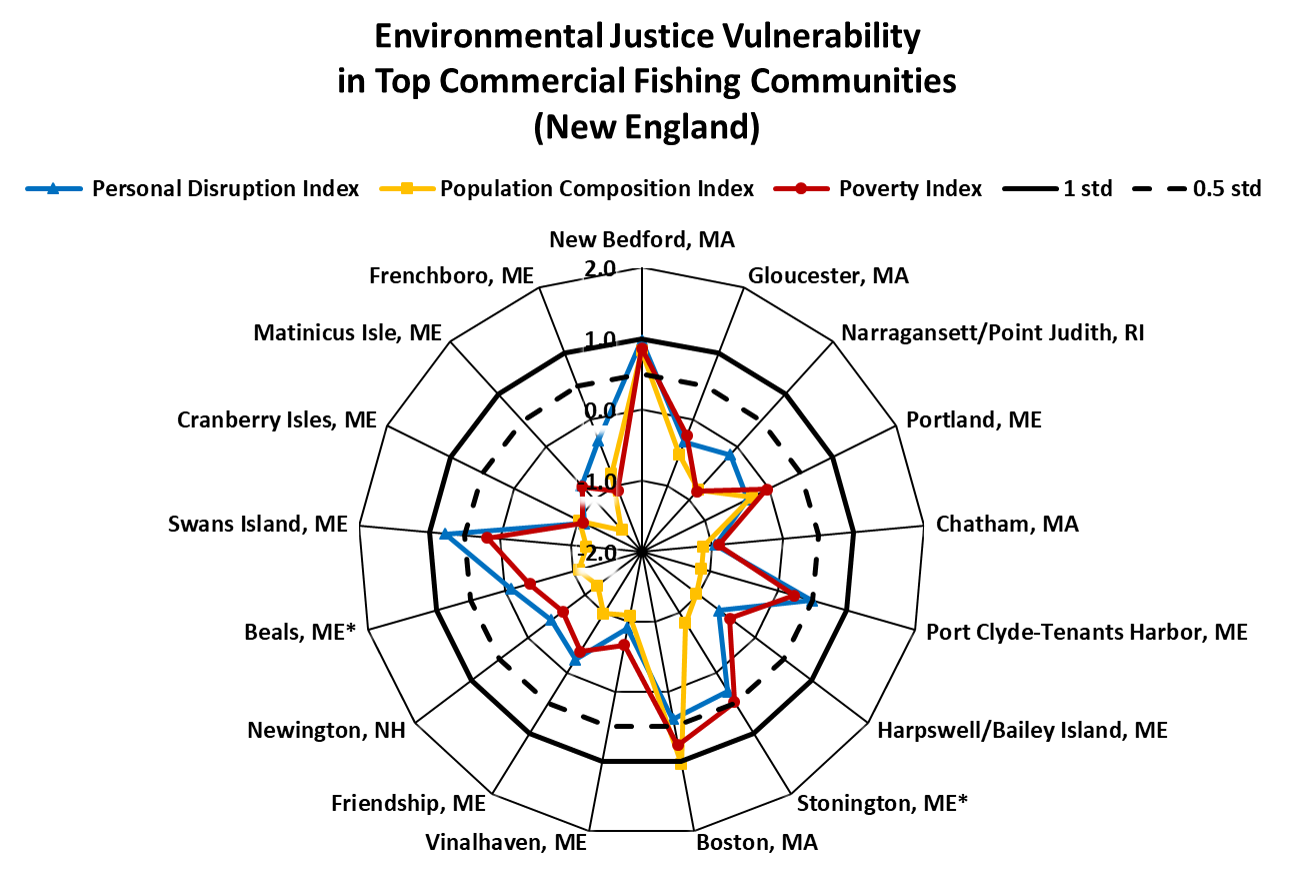
\includegraphics[width=0.7\linewidth]{SOE-NEFMC_files/figure-latex/commercial-EJ-1} 

}

\caption{Environmental justice indicators (Poverty Index, population composition index, and personal disruption index) for top commercial fishing communities in New England. *Community scored high (1.00 and above) for both commercial engagement and reliance indicators.}\label{fig:commercial-EJ}
\end{figure}
\begin{figure}

{\centering \includegraphics{SOE-NEFMC_files/figure-latex/recreational-engagement-1} 

}

\caption{Recreational engagement and reliance, and environmental justice vulnerability, for the top recreationally engaged and reliant fishing communities in New England. None of these communities ranked medium-high or above for one or more of the environmental justice indicators. Communities ranked medium for one or more of the environmental justice indicators are highlighted in purple. *Community scored high (1.00 and above) for both recreational engagement and reliance indicators.}\label{fig:recreational-engagement}
\end{figure}
\begin{figure}

{\centering 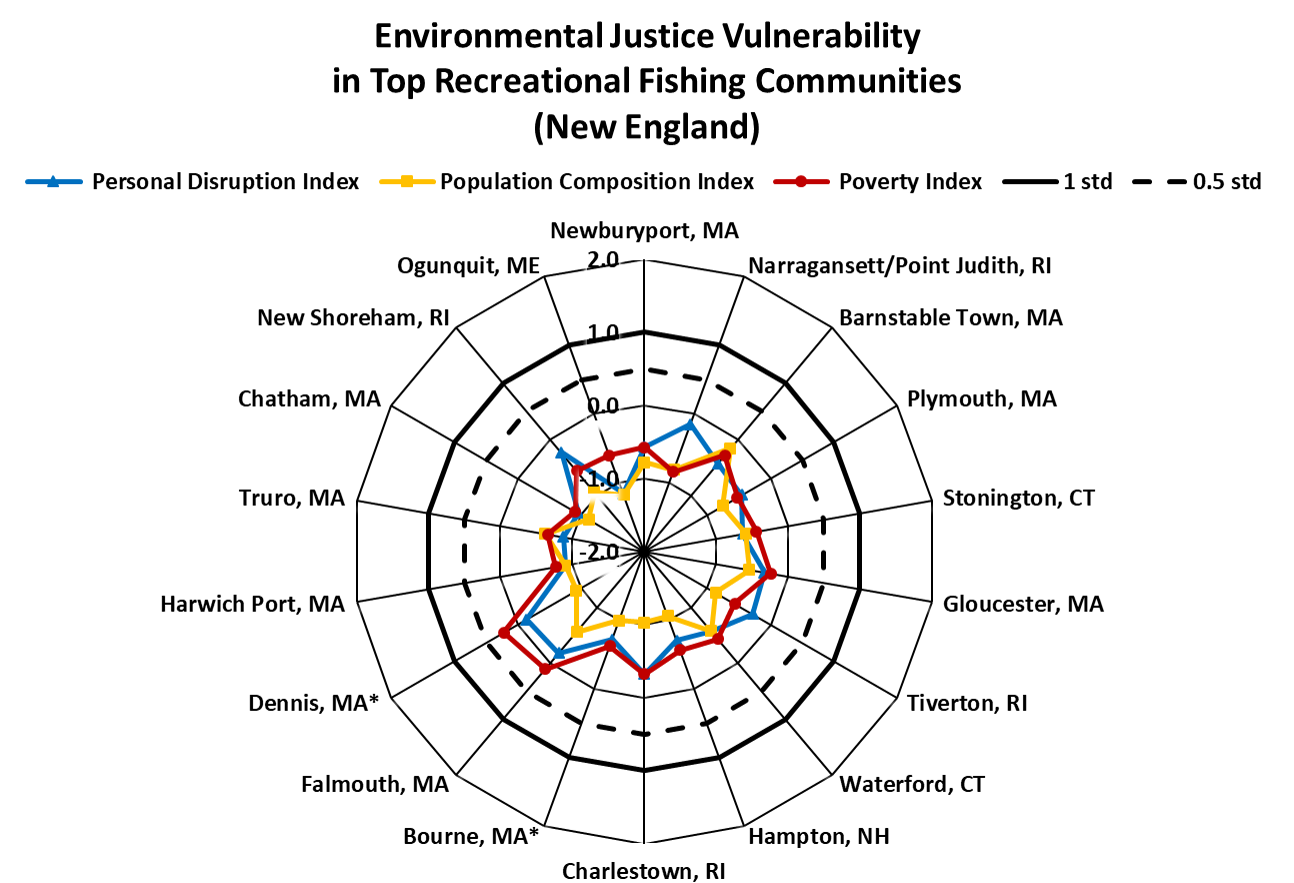
\includegraphics[width=0.75\linewidth]{SOE-NEFMC_files/figure-latex/recreational-EJ-1} 

}

\caption{Environmental justice indicators (Poverty Index, population composition index, and personal disruption index) for top recreational fishing communities in New England. *Community scored high (1.00 and above) for both commercial engagement and reliance indicators.}\label{fig:recreational-EJ}
\end{figure}

Both commercial and recreational fishing are important activities in Narragansett/Point Judith, RI; Gloucester and Chatham, MA, meaning these communities may be impacted simultaneously by commercial and recreational regulatory changes. These three communities currently score low for all of the three environmental justice indicators, indicating that environmental justice may not be a major concern in these communities at the moment based on the indicators analyzed.

\hypertarget{implications-4}{%
\subsubsection{Implications}\label{implications-4}}

These indicators provide a snapshot of the presence of environmental justice issues in the most highly engaged and most highly reliant commercial and recreational fishing communities in New England. These communities may be especially vulnerable to changes in fishing patterns due to regulations and/or climate change. A range of environmental justice concerns are found throughout Mid-Atlantic fishing communities. However, index scores for these concerns are higher overall in the top commercial communities relative to the top recreational communities. Some changes occurred among the top recreational fishing communities between 2020 and 2021 due to shifts in recreational fishing activities, while the top commercial communities remained stable. A few of these top fishing communities, mostly commercial fishing communities, demonstrated medium to high environmental justice vulnerability, indicating that they may be at a disadvantage responding to change.
\#\# Protected Species

Fishery management objectives for protected species generally focus on reducing threats and on habitat conservation/restoration. Protected species include marine mammals protected under the Marine Mammal Protection Act, endangered and threatened species protected under the Endangered Species Act, and migratory birds protected under the Migratory Bird Treaty Act. In the Northeast U.S., endangered/threatened species include Atlantic salmon, Atlantic and shortnose sturgeon, all sea turtle species, and five baleen whales. Here we report on the status of these actions as well as indicating the potential for future interactions driven by observed and predicted ecosystem changes in the Northeast U.S. Protected species objectives include managing bycatch to remain below potential biological removal (PBR) thresholds, recovering endangered populations, and monitoring unusual mortality events (UMEs).

\hypertarget{indicators-bycatch-population-adult-and-juvenile-numbers-mortalities}{%
\subsubsection{Indicators: bycatch, population (adult and juvenile) numbers, mortalities}\label{indicators-bycatch-population-adult-and-juvenile-numbers-mortalities}}

Average indices for both \href{https://noaa-edab.github.io/catalog/harbor-porpoise-bycatch.html}{harbor porpoise} (Fig. \ref{fig:harborporpoise}) and \href{https://noaa-edab.github.io/catalog/gray-seal-bycatch.html}{gray seal} bycatch (Fig. \ref{fig:grayseal}) are below current PBR thresholds, meeting management objectives.

\begin{figure}

{\centering \includegraphics{SOE-NEFMC_files/figure-latex/harborporpoise-1} 

}

\caption{Harbor porpoise average bycatch estimate for Mid-Atlantic and New England gillnet fisheries (blue) and the potential biological removal (red).}\label{fig:harborporpoise}
\end{figure}
\begin{figure}

{\centering \includegraphics{SOE-NEFMC_files/figure-latex/grayseal-1} 

}

\caption{Gray Seal average bycatch estimate for gillnet fisheries (blue) and the potential biological removal (red).}\label{fig:grayseal}
\end{figure}

The annual estimate for gray seal bycatch has declined since 2019, in part driven by declining gillnet landings. In addition, estimates since 2019 have greater uncertainty stemming from low observer coverage since 2019. The rolling mean confidence interval remains just below the PBR value.

The \href{https://noaa-edab.github.io/catalog/right-whale-abundance.html}{North Atlantic right whale population} was on a recovery trajectory until 2010, but has since declined (Fig. \ref{fig:narw-abundance}). The sharp decline observed from 2015-2020 appears to have slowed, although the right whale population continues to experience annual mortalities above recovery thresholds. Reduced survival rates of adult females lead to diverging abundance trends between sexes. It is estimated that there are fewer than 70 adult females remaining in the population.

\begin{figure}

{\centering \includegraphics{SOE-NEFMC_files/figure-latex/narw-abundance-1} 

}

\caption{Estimated North Atlanic right whale abundance on the Northeast Shelf.}\label{fig:narw-abundance}
\end{figure}

North Atlantic right whale \href{https://noaa-edab.github.io/catalog/right-whale-abundance.html}{calf counts} have generally declined after 2009 to the point of having zero new calves observed in 2018 (Fig. \ref{fig:NARW-calf-abundance}). However, since 2019, we have seen more calf births each year with 15 births in 2022.

This year, the Unusual Mortality Event (UME) for North Atlantic right whales continued. Since 2017, the total UME right whale mortalities includes 36 dead stranded whales, 15 in the U.S. and 21 in Canada. When alive but seriously injured whales (35) and sublethal injuries or ill whales (51) are taken into account, 122 individual whales are included in the UME. Recent research suggests that many mortalities go unobserved and the true number of mortalities are about three times the count of the observed mortalities. The primary cause of death is ``human interaction'' from entanglements or vessel strikes.

A UME continued from previous years for humpback whales (2016-present); suspected causes include human interactions. A UME for both gray and harbor seals on the Maine coast was declared in June 2022 due to a high number of mortalities thought to be caused by highly pathogenic avian influenza virus. A UME for minke whales that began in 2017 remains open, but is pending closure as of January 2024.

\begin{figure}

{\centering \includegraphics{SOE-NEFMC_files/figure-latex/NARW-calf-abundance-1} 

}

\caption{Number of North Atlantic right whale calf births, 1990 - 2021.}\label{fig:NARW-calf-abundance}
\end{figure}

\hypertarget{implications-5}{%
\subsubsection{Implications}\label{implications-5}}

Bycatch management measures have been implemented to maintain bycatch below PBR thresholds. The downward trend in harbor porpoise bycatch can also be due to a decrease in harbor porpoise abundance in U.S. waters, reducing their overlap with fisheries, and a decrease in gillnet effort. The increasing trend in gray seal bycatch may be related to an increase in the gray seal population (\href{https://noaa-edab.github.io/catalog/gray-seal-pups.html}{U.S. pup counts}), supported by the dramatic rise over the last three decades in observed numbers of gray seal pups born at U.S. breeding sites plus an increase in adult seals at the breeding sites (Fig. \ref{fig:seals}), some of which are supplemented by Canadian adults.

\begin{figure}

{\centering \includegraphics{SOE-NEFMC_files/figure-latex/seals-1} 

}

\caption{Estimated mean rates of increase in the number of gray seal pups born at four United States pupping colonies at various times from 1988 to 2021. Recreated from Wood et al. 2022 (Figure 5).}\label{fig:seals}
\end{figure}

Strong evidence exists to suggest that interactions between right whales and both the fixed gear fisheries in the U.S. and Canada and vessel strikes in the U.S. are contributing substantially to the decline of the species. Further, right whale distribution has changed since 2010. \href{https://noaa-edab.github.io/catalog/right-whale-abundance.html}{New research} suggests that recent climate driven changes in ocean circulation have resulted in right whale distribution changes driven by increased warm water influx through the Northeast Channel, which has reduced the primary right whale prey (Calanus finmarchicus) in the central and eastern portions of the Gulf of Maine. Additional potential stressors include offshore wind development, which overlaps with important habitat areas used year-round by right whales, including mother and calf migration corridors and foraging habitat. This area is also a primary right whale winter foraging habitat. Additional information can be found in the \protect\hyperlink{other-ocean-uses:-offshore-wind}{offshore wind risks section}.

The UMEs are under investigation and are likely the result of multiple drivers. For all large whale UMEs, human interaction appears to have contributed to increased mortalities, although investigations are not complete.

A climate vulnerability assessment is published for Atlantic and Gulf of Mexico marine mammal populations.

\newpage

\hypertarget{risks-to-meeting-fishery-management-objectives}{%
\section{Risks to meeting fishery management objectives}\label{risks-to-meeting-fishery-management-objectives}}

\hypertarget{climate-and-ecosystem-change}{%
\subsection{Climate and Ecosystem Change}\label{climate-and-ecosystem-change}}

Regulations and measures designed to meet fishery management objectives are often based on historical information about stocks, their distribution in space and time, and their overall productivity. Large scale climate related changes in the ecosystem can lead to changes in important habitats and ecological interactions, altering distributions and productivity. With large enough ecosystem changes, management measures may be less effective and management objectives may not be met.

This year, we restructured this section to focus on three categories of management decisions and the risk posed to them by climate and ecosystem change: spatial management, seasonal management, and quota setting or rebuilding depleted stocks. In each section, we describe potential risks to the management category, highlight indicators of observed changes that contribute to those risks, and review possible biological and environmental drivers and the ways they may explain the observed indicators.

\hypertarget{risks-to-spatial-management}{%
\subsubsection{Risks to Spatial Management}\label{risks-to-spatial-management}}

Shifting species distributions (changes in spatial extent or center of gravity) alter both species interactions and fishery interactions. In particular, shifting species distributions can affect expected management outcomes from spatial allocations and bycatch measures based on historical fish and protected species distributions. Additionally, species availability to surveys can change as distributions shift within survey footprints.

\hypertarget{indicator-fish-and-protected-species-distribution-shifts}{%
\paragraph{Indicator: Fish and protected species distribution shifts}\label{indicator-fish-and-protected-species-distribution-shifts}}

As noted in the landings Implications section above, the center of distribution for a suite of 48 commercially or ecologically important fish species along the entire Northeast Shelf continues to show movement towards the northeast and generally into deeper water (Fig.\ref{fig:protectedspp-dist-shifts} ). \href{https://noaa-edab.github.io/catalog/species-richness.html}{Habitat model-based species richness} suggests shifts of both cooler and warmer water species to the northeast. Similar patterns have been found for \href{https://noaa-edab.github.io/catalog/cetacean-distribution-shifts.html}{marine mammals}, with multiple species shifting northeast between 2010 and 2017 in most seasons (Fig. \ref{fig:species-dist} ).

\begin{figure}

{\centering \includegraphics{SOE-NEFMC_files/figure-latex/protectedspp-dist-shifts-1} 

}

\caption{Direction and magnitude of core habitat shifts, represented by the length of the line of the seasonal weighted centroid for species with more than 70 km difference between 2010 and 2017 (tip of arrow).}\label{fig:protectedspp-dist-shifts}
\end{figure}

\hypertarget{drivers}{%
\paragraph{Drivers}\label{drivers}}

Mobile populations are shifting distributions to maintain suitable temperature and prey fields, possibly expanding if new suitable habitat exists. Changes in managed species distribution is related, in part, to the \href{https://noaa-edab.github.io/catalog/forage-fish-index.html}{distribution of forage biomass}. Since 1982, the fall center of gravity of forage fish (20 species combined) has moved to the north and east. Spring forage fish center of gravity has been more variable over time.

\begin{figure}

{\centering \includegraphics{SOE-NEFMC_files/figure-latex/species-dist-1} 

}

\caption{Aggregate species distribution metrics for species in the Northeast Large Marine Ecosystem.}\label{fig:species-dist}
\end{figure}
\begin{figure}

{\centering \includegraphics{SOE-NEFMC_files/figure-latex/forage-cog-1} 

}

\caption{Eastward (left) and northward (right) shifts in the center of gravity for 20 forage fish species on the Northeast U.S. Shelf.}\label{fig:forage-cog}
\end{figure}

Ocean temperatures influence the distribution, seasonal timing, and productivity of managed species (see sections below). New England has experienced a continued warming trend for both the \href{https://noaa-edab.github.io/catalog/sea-surface-temperature-anomaly.html}{surface} (Fig.\ref{fig:longterm-sst}) and \href{https://noaa-edab.github.io/catalog/bottom-temperature---seasonal-anomaly.html}{bottom} (Fig. \ref{fig:bottom-temp}) in all seasons.

\begin{figure}

{\centering \includegraphics{SOE-NEFMC_files/figure-latex/longterm-sst-1} 

}

\caption{Mean sea surface temperature across the entire Mid-Atlantic shelf.}\label{fig:longterm-sst}
\end{figure}

Species suitable habitat can expand or contract when changes in temperature and major oceanographic conditions alter distinct water mass habitats. The variability of the Gulf Stream is a major driver of the predominant oceanographic conditions of the Northeast U.S. continental shelf. As the \href{https://noaa-edab.github.io/catalog/gulf-stream-index.html}{Gulf Stream} has become less stable and shifted northward in the last decade (Fig. \ref{fig:GSI}), warmer ocean temperatures have been observed on the northeast shelf and a higher proportion of \href{https://noaa-edab.github.io/catalog/slopewater-proportions.html}{Warm Slope Water} has been present in the Gulf of Maine Northeast Channel. Since 2008, the Gulf Stream has moved closer to the Grand Banks, reducing the supply of cold, fresh, and oxygen-rich Labrador Current waters to the Northwest Atlantic Shelf. Nearly every year since 2010, warm slope water made up more than 50\% of the annual slope water proportions entering the Gulf of Maine. In 2017 almost no cooler Labrador Slope water entered the Gulf of Maine through the Northeast Channel. The changing proportions of source water affect the temperature, salinity, and nutrient inputs to the Gulf of Maine ecosystem. In 2022, warm slope water was a majority (59.7\%) of inputs to the Gulf of Maine.

\begin{figure}

{\centering \includegraphics{SOE-NEFMC_files/figure-latex/GSI-1} 

}

\caption{Index representing changes in the location of the Gulf Stream north wall. Positive values represent a more northerly Gulf Stream position.}\label{fig:GSI}
\end{figure}

\hypertarget{future-considerations}{%
\paragraph{Future Considerations}\label{future-considerations}}

Distribution shifts caused by changes in thermal habitat are likely to continue as long as long-term temperature trends persist. Near-term oceanographic forecasts are currently in development and may inform how future warming impacts species distributions.

Distribution patterns associated with climate-driven changes in oceanographic circulation patterns are unlikely to be reversed to historical ranges in the short term. Increased oceanographic variability needs to be captured by regional ocean models and linked to species distribution processes to better understand potential future distributions. Species with high mobility or short life spans react differently from immobile or long lived species.

Adapting management to changing stock distributions and dynamic ocean processes will require continued monitoring of populations in space and evaluating management measures against a range of possible future spatial distributions.

\hypertarget{risks-to-seasonal-management}{%
\subsubsection{Risks to Seasonal Management}\label{risks-to-seasonal-management}}

The effectiveness of seasonal management actions (fishing seasons or area opening/closing) depends on a proper alignment with the seasonal life cycle events, also known as phenology, of fish stocks (e.g.~migration timing and spawning). Changes in the timing of these biological cycles can reduce the effectiveness of management measures if not accounted for. The timing of seasonal patterns can also change the availability of species to surveys and interactions between fisheries of non-target species thus influencing the amount of bycatch.

\hypertarget{indicators-timing-shifts}{%
\paragraph{Indicators: Timing shifts}\label{indicators-timing-shifts}}

\href{https://noaa-edab.github.io/catalog/spawning-timing.html}{Spawning timing} is shifting earlier for multiple stocks, including haddock and yellowtail flounder (Fig. \ref{fig:spawn-timing}). Spawning of both haddock stocks is occurring earlier, as indicated by more resting (post-spawning) stage fish in the 2010s as compared to earlier in the time series. The northern (Cape Cod/GOM) stock shows earlier active spawning in recent years with a decline in pre-spawning resting females. Yellowtail flounder spawning is related to bottom temperature, week of year, and decade sampled for each of the three stocks.

\begin{figure}

{\centering \includegraphics{SOE-NEFMC_files/figure-latex/spawn-timing-1} 

}

\caption{Percent resting stage (non-spawning) fish from two haddock and three yellowtail flounder stocks: CC = Cape Cod Gulf of Maine, GOM = Gulf of Maine, GB = Georges Bank, SNE = Southern New England.}\label{fig:spawn-timing}
\end{figure}

\href{https://noaa-edab.github.io/catalog/timing-shifts-risks-to-seasonal-management.html}{Migration timing} of some tuna and large whale migrations has changed. For example, tuna were caught in recreational fisheries 50 days earlier in the year in 2019 compared to 2002. In Cape Cod Bay, peak spring habitat use by right and humpback whales has shifted 18-19 days later over time.

Understanding whether seasonal patterns are changing for stocks requires regular observations during those events. Despite the importance of understanding seasonal patterns, we have few indicators that directly assess timing shifts of species. We plan on incorporating more indicators of phenology in future reports.

\hypertarget{drivers-1}{%
\paragraph{Drivers}\label{drivers-1}}

The drivers of timing shifts in managed stocks are generally coupled to shifts in environmental or biological conditions, since these can result in changes in habitat quality or food availability within the year. Changes in the timing of fall phytoplankton blooms and seasonal shifts in zooplankton communities are thought to be critical indicators of changes in seasonal food availability to stocks.

Along with the overall warming trends in New England, ocean summer conditions have been lasting longer, as shown by the later \href{https://noaa-edab.github.io/catalog/transition-dates.html}{transition} from warm stratified summer conditions to well mixed cool fall conditions (Fig. \ref{fig:transition}). Changes in the broad seasonal cycles of their environment can lead to changes in species biological processes (migrations, spawning, etc.) that are triggered by seasonal events. Additionally, prolonged fall temperatures have been linked to the increased number of cold-stunned Kemp's ridley sea turtles found in Cape Cod Bay.

\begin{figure}

{\centering \includegraphics{SOE-NEFMC_files/figure-latex/transition-1} 

}

\caption{Ocean summer length: the annual total number of days between the spring thermal transition date and the fall thermal transition date. The transition dates are defined as the day of the year when surface temperatures change from cool to warm conditions in the spring and back to cool conditions in the fall.}\label{fig:transition}
\end{figure}

The \href{https://noaa-edab.github.io/catalog/cold-pool-index.html}{cold pool} is a seasonal feature within the MAB that creates seasonally suitable habitat for many species. Since the mid-2000s, the cold pool has persisted for a shorter portion of the year (Fig. \ref{fig:cold-pool-time}). A change in the timing of the cold pool may impact the recruitment of species that utilize it for seasonal cues. Southern New England-Mid Atlantic yellowtail flounder recruitment and settlement are related to the strength of the cold pool (a factor of extent and persistence). The dependency of pre-recruit settlers within the cold pool represents a bottleneck in yellowtail life history, during which a local and temporary increase in bottom temperature negatively impacts the survival of the settlers. Including the effect of cold pool variations on yellowtail recruitment reduced retrospective patterns and improved the skill of short-term forecasts in a stock assessment model.

\begin{figure}

{\centering \includegraphics{SOE-NEFMC_files/figure-latex/cold-pool-time-1} 

}

\caption{Seasonal cold pool annual duration. Open circles represent data derived from ROMS -NWA and closed circle data are derived from GLORYS.}\label{fig:cold-pool-time}
\end{figure}

\hypertarget{future-considerations-1}{%
\paragraph{Future Considerations}\label{future-considerations-1}}

For stocks reliant on environmental processes to dictate the timing of their behavior (e.g.~phytoplankton bloom timing, thermal transition, or the duration of the cold pool), it is possible that some effects will be episodic and have interannual variability, while other effects on timing can change on scales of years to decades. However, other species rely on the general seasonal succession of environmental drivers (e.g.~the timing of the fall turnover) to cue biological processes, which rely on long-term trends unlikely to reverse in coming years. Such timing shifts in migration or spawning for those species are expected to continue. Management actions that rely on effective alignment of fisheries availability and biological processes should continue to evaluate whether prior assumptions on seasonal timings still hold, and new indicators should be developed to monitor timing shifts for stocks.

\hypertarget{risks-to-quota-settingrebuilding}{%
\subsubsection{Risks to Quota Setting/Rebuilding}\label{risks-to-quota-settingrebuilding}}

The efficacy of short-term stock projections and rebuilding plans rely on an accurate understanding of processes affecting stock growth, reproduction, and natural mortality. These biological processes are often driven by underlying environmental change. When observed environmental change occurs, there is a risk that established stock-level biological reference points may no longer reflect the current population.

\hypertarget{indicators-fish-productivity-and-condition-shifts}{%
\paragraph{Indicators: Fish productivity and condition shifts}\label{indicators-fish-productivity-and-condition-shifts}}

Indicators of \href{https://noaa-edab.github.io/catalog/fish-productivity-indicators.html}{fish productivity} are derived from observations (surveys) or models (stock assessments). With the exception of two years (2006 and 2013), fish productivity has been below the long-term average in the Gulf of Maine since the early 2000s, as described by the small-fish-per-large-fish anomaly indicator (derived from NEFSC bottom trawl survey)(Fig. \ref{fig:productivity-anomaly}). This decline in fish productivity is also shown by a similar analysis based on stock assessment model outputs (recruitment per spawning stock biomass anomaly). Other signs of changing productivity in New England are the declines in \href{https://noaa-edab.github.io/catalog/seabird-diet-and-productivity---new-england.html}{common tern chicks} per nest (Fig. \ref{fig:seabird-ne-productivity}) and declining return rates for \href{https://noaa-edab.github.io/catalog/gulf-of-maine-atlantic-salmon.html}{Atlantic salmon}(Fig. \ref{fig:salmon}).

\begin{figure}

{\centering \includegraphics{SOE-NEFMC_files/figure-latex/productivity-anomaly-1} 

}

\caption{Fish productivity measures. Left: Small fish per large fish survey biomass anomaly in the Gulf of Maine. Right: assessment recruitment per spawning stock biomass anomaly for stocks managed by the New England Fishery Management Council region. The summed anomaly across species is shown by the black line, drawn across all years with the same number of stocks analyzed.}\label{fig:productivity-anomaly}
\end{figure}
\begin{figure}

{\centering \includegraphics{SOE-NEFMC_files/figure-latex/seabird-ne-productivity-1} 

}

\caption{Productivity of Common terns in the Gulf of Maine.}\label{fig:seabird-ne-productivity}
\end{figure}
\begin{figure}

{\centering \includegraphics{SOE-NEFMC_files/figure-latex/salmon-1} 

}

\caption{Return rate proportions and abundance of Atlantic salmon.}\label{fig:salmon}
\end{figure}

The health of individual fish (i.e.~fish condition) can contribute to population productivity through improved growth, reproduction and survival. \href{https://noaa-edab.github.io/catalog/relative-condition.html}{Fish condition} in the Gulf of Maine and Georges Bank regions were generally good prior to 2000, poor from 2001-2010 (concurrent with declines in fish productivity, Fig. \ref{fig:productivity-anomaly}), and a mix of good and poor since 2011. In 2023, fish condition was mixed, with generally improving condition on Georges Bank, but the highest number of species in poor condition in the Gulf of Maine since 2010 (Fig. \ref{fig:ne-cf}).

\begin{figure}

{\centering \includegraphics{SOE-NEFMC_files/figure-latex/ne-cf-1} 

}

\caption{Condition factor for fish species in New England based on fall NEFSC bottom trawl survey data. No survey was conducted in 2020.}\label{fig:ne-cf}
\end{figure}

\hypertarget{drivers-2}{%
\paragraph{Drivers}\label{drivers-2}}

Fish productivity and condition are affected by increasing metabolic demands from increasing temperature, combined with changes in the availability and quality of prey. Long-term environmental trends and episodic extreme temperatures, ocean acidification, and low oxygen events represent multiple stressors that can affect growth rates, reproductive success, recruitment, and cause mortality.

\hypertarget{biological-drivers-forage-quality-and-abundance}{%
\subparagraph{Biological Drivers: Forage quality and abundance}\label{biological-drivers-forage-quality-and-abundance}}

Fish productivity is dependent on the energy potentially available to them based on the nutritional value (energy content) and abundance of prey. Changes in the forage fish base can drive managed and protected species production and condition.

The \href{https://noaa-edab.github.io/catalog/forage-fish-energy-density.html}{energy content} of juvenile and adult forage fish as prey is related to forage fish growth and reproductive cycles, as well as environmental conditions. The energy content of Atlantic herring from the NEFSC trawl surveys has increased but is still well below observations in the 1980s and 1990s (Fig. \ref{fig:energy-density}). Silver hake, longfin squid (Loligo in figure) and shortfin squid (Illex in figure) remain lower than previous estimates.

\begin{figure}

{\centering \includegraphics{SOE-NEFMC_files/figure-latex/energy-density-1} 

}

\caption{Forage fish energy density mean and standard deviation by season and year, compared with 1980s (solid line; Steimle and Terranove 1985) and 1990s (dashed line; Lawson et al. 1998) values.}\label{fig:energy-density}
\end{figure}

Changes in the overall abundance of forage fish can influence managed species productivity as it relates to changes in food availability. New England \href{https://noaa-edab.github.io/catalog/forage-fish-index.html}{fall forage biomass} is stable with long-term increases in the spring GOM(Fig. \ref{fig:foragebio}). Forage biomass was highest during fall in the 1980s.

\hypertarget{biological-drivers-lower-trophic-levels}{%
\subparagraph{Biological Drivers: Lower trophic levels}\label{biological-drivers-lower-trophic-levels}}

Phytoplankton are the foundation of the food web and are the primary food source for zooplankton and filter feeders such as shellfish. Numerous environmental and oceanographic factors interact to drive the abundance, composition, spatial distribution, and productivity of phytoplankton. While changes in fish productivity (including forage) could result from changing primary productivity, total primary production in New England has no long-term trend, despite anomalous conditions in the GOM in 2023 (Fig. \ref{fig:primaray-production}).

Since 2010, the abundance of the lipid-rich older stages of \href{https://noaa-edab.github.io/catalog/mesozooplankton-biomass-at-wilkson-basin.html}{\emph{Calanus finmarchicus}} in the GOM has declined. Observations from a fixed time series station in Wilkinson Basin indicate that \href{https://noaa-edab.github.io/catalog/seasonal-variation-of-calanus-finmarchicus.html}{\emph{Calanus} abundance} in late summer-winter between 2020-2022 has declined to 30-40\% of its population level in 2005-2008, although spring abundances are still the same as 15-20 years ago. The seasonal differences in abundance change reflect differences in influence of primary seasonal drivers:

\begin{enumerate}
\def\labelenumi{\arabic{enumi}.}
\tightlist
\item
  \emph{Calanus} reproductive output is tied to phytoplankton availability in late winter/early spring.
\item
  Gulf of Maine source waters drive \emph{Calanus} supply (high \emph{Calanus} in Scotian Shelf/ LSW and less in WSW)
\item
  Predation is likely higher with warmer temperatures
\end{enumerate}

\begin{figure}

{\centering \includegraphics{SOE-NEFMC_files/figure-latex/foragebio-1} 

}

\caption{Forage fish index in GB (left) and GOM (right) for spring (blue) and fall (red) surveys. Index values are relative to the maximum observation within a region across surveys.}\label{fig:foragebio}
\end{figure}
\begin{figure}

{\centering 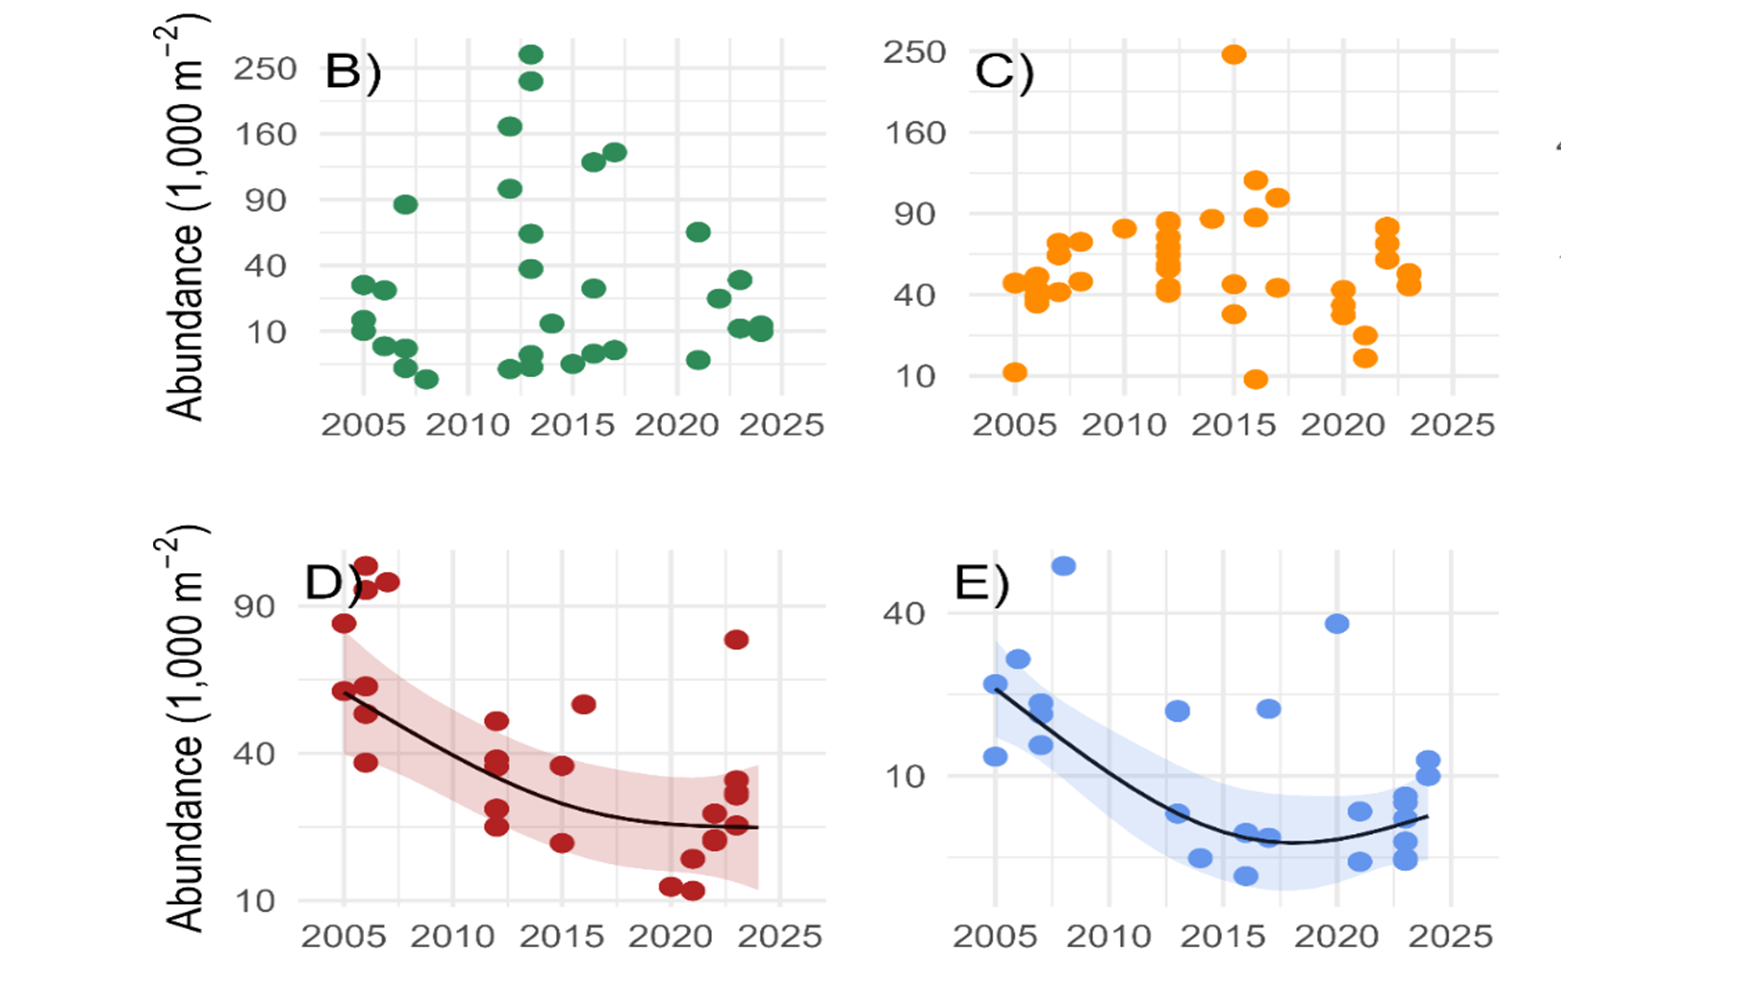
\includegraphics{SOE-NEFMC_files/figure-latex/zooplankton-season-1} 

}

\caption{Seasonal indices of dry mass of mesozooplankton captured with a 200µm ring net towed from the bottom to surface at a deep time series station  in Wilkinson Basin between 2005-2022 (Runge et al. 2023).}\label{fig:zooplankton-season}
\end{figure}
\begin{figure}

{\centering \includegraphics{SOE-NEFMC_files/figure-latex/zoo-abund-1} 

}

\caption{Georges Bank (GB) and Gulf of Maine (GOM) abundance anomalies three dominante zooplankton (\textit{Calanus finmarchicus}, \textit{Calanus typicus}, and \textit{Pseudocalanus spp}.).}\label{fig:zoo-abund}
\end{figure}

\hypertarget{environmental-drivers}{%
\subparagraph{Environmental Drivers}\label{environmental-drivers}}

Fish production can also be directly related to the prevailing environmental conditions by altering metabolic (growth) and reproductive processes. Many species possess thermal tolerances and can experience stressful or lethal conditions if temperatures exceed certain levels. Extreme temperature at both the \href{https://noaa-edab.github.io/catalog/sea-surface-temperature-anomaly.html}{surface} (Fig. \ref{fig:longterm-sst}) and \href{https://noaa-edab.github.io/catalog/bottom-temperature---seasonal-anomaly.html}{bottom} can exceed \href{https://noaa-edab.github.io/catalog/thermal-habitat-persistence.html}{thermal tolerance} limits for some fish. For example, 2012 had among the warmest surface and bottom temperatures in New England. A large proportion of the Georges Bank and Mid-Atlantic regions had bottom temperatures above the 15℃ thermal tolerance for most groundfish, with some days exceeding the 24℃ potential mortality limit (Fig. \ref{fig:therm-hab-persist-2012}). The second strongest \href{https://noaa-edab.github.io/catalog/marine-heatwaves---bottom.html}{bottom marine heatwave} since 1982 was observed in the GOM, although it did not exceed this 15℃ threshold. Most of GB and the inshore GOM have exceeded this 15℃ threshold since 2012.

\begin{figure}

{\centering 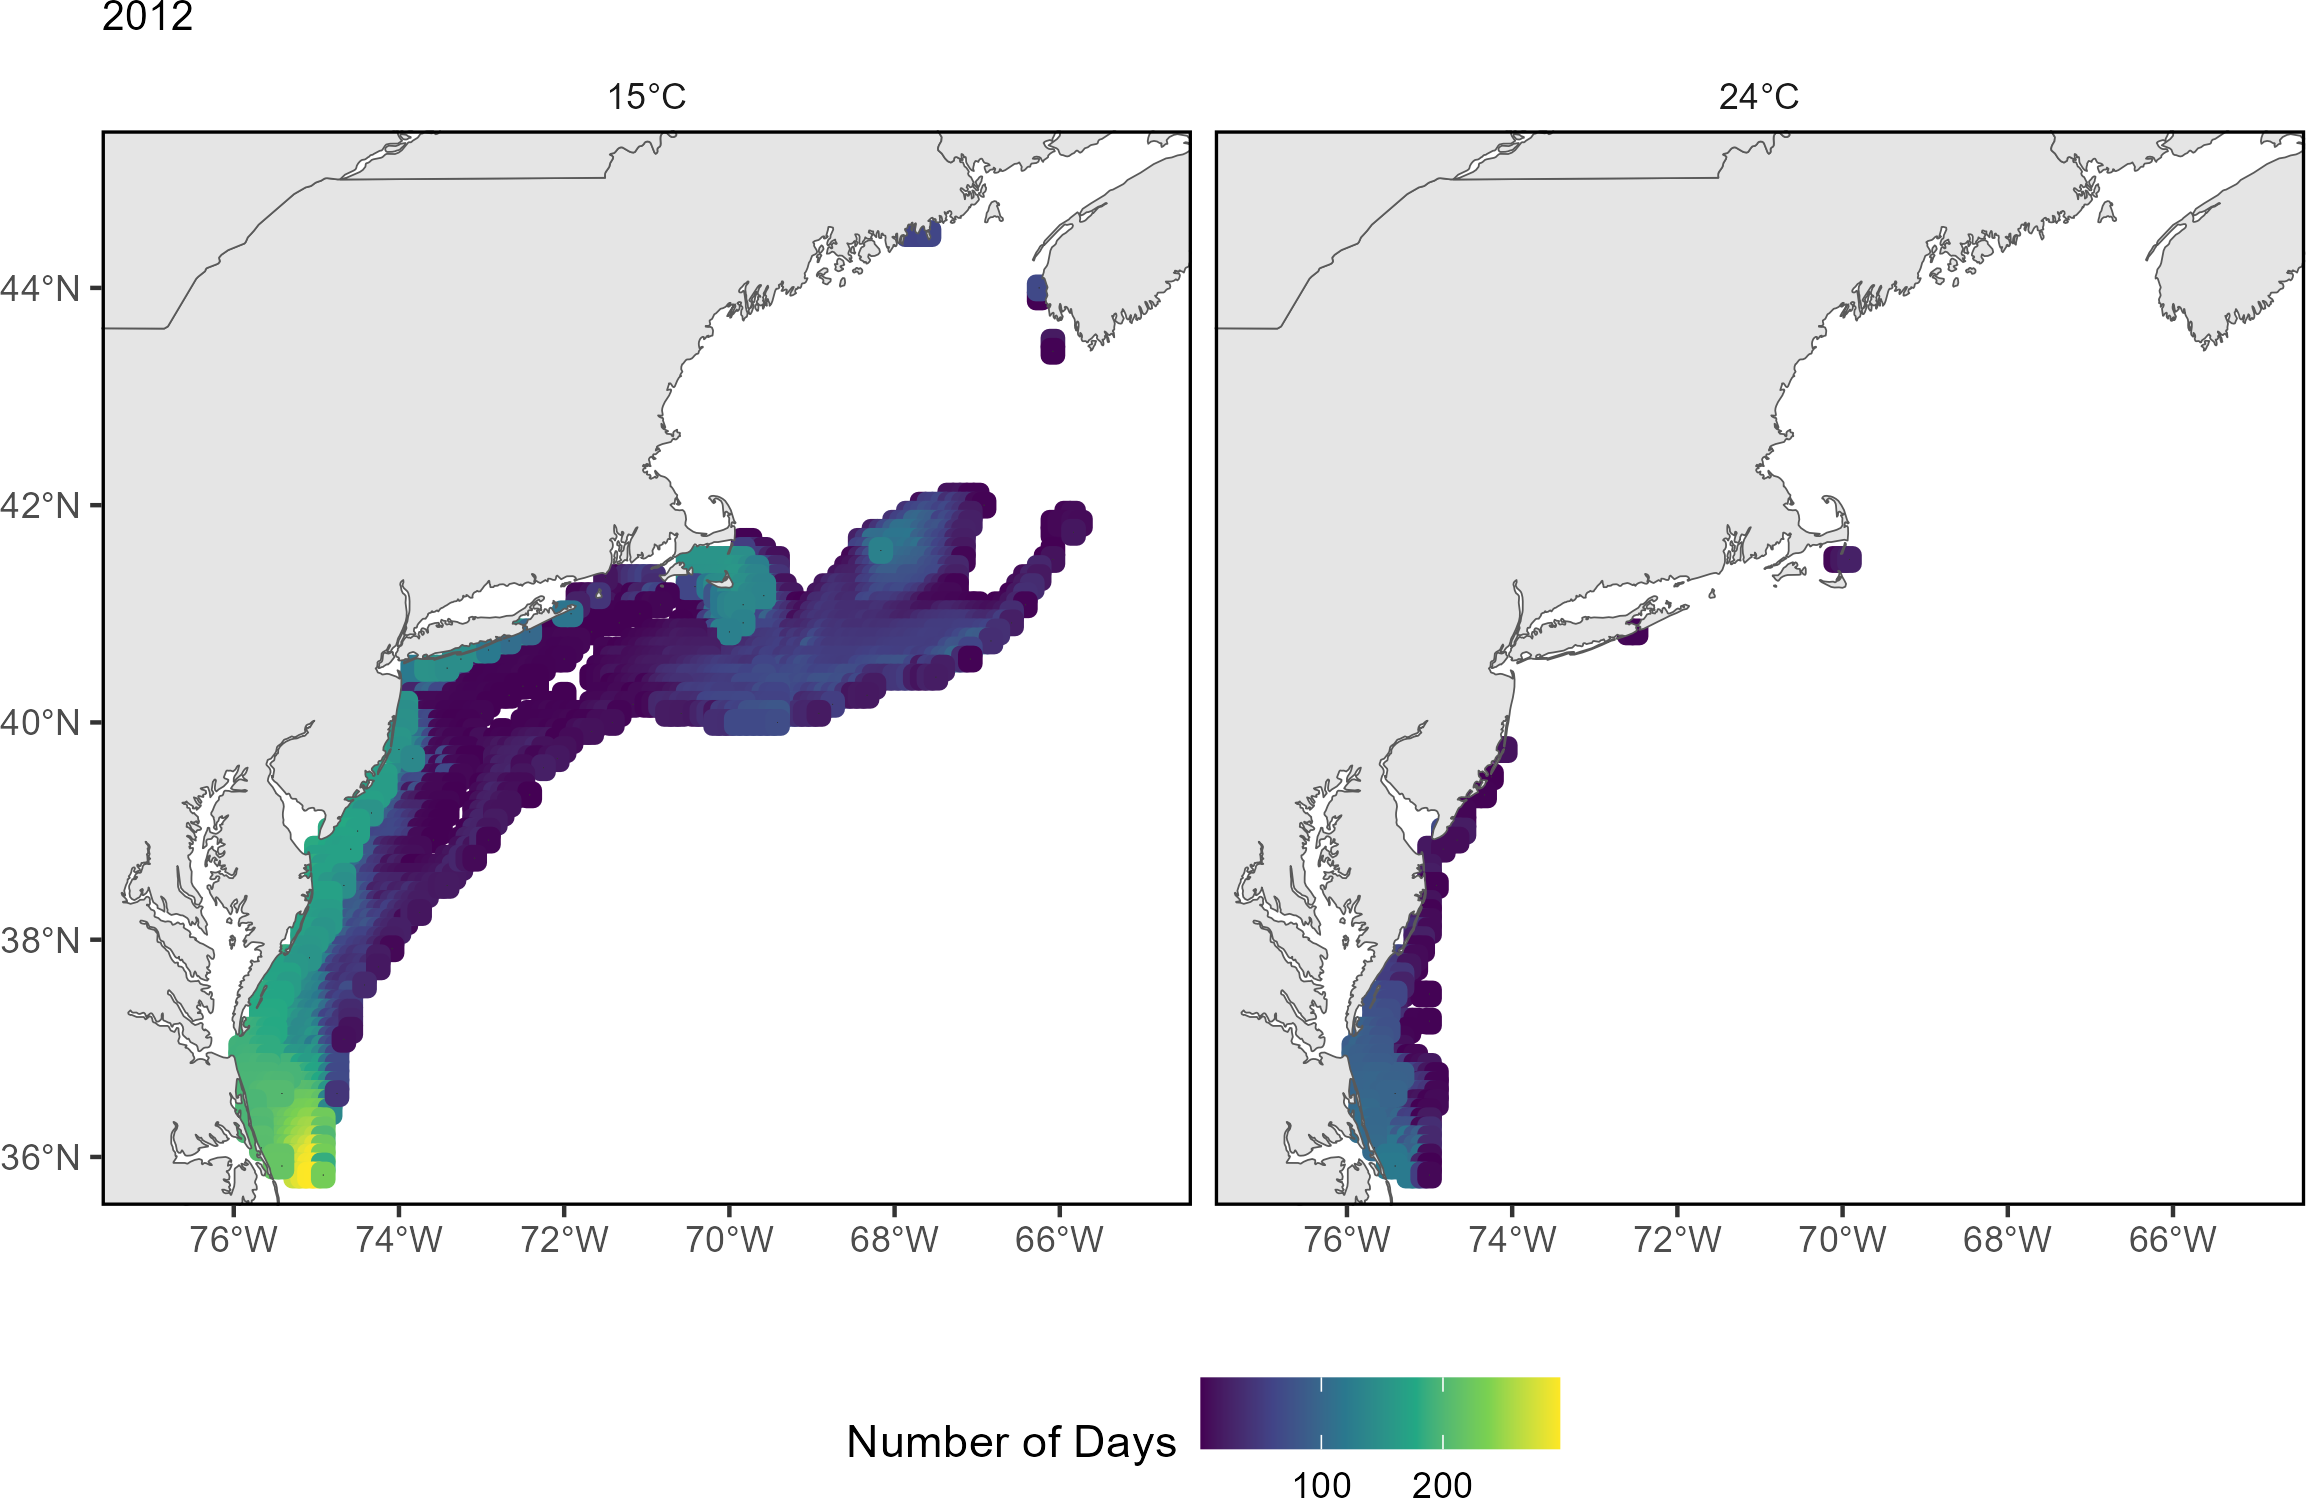
\includegraphics{SOE-NEFMC_files/figure-latex/therm-hab-persist-2012-1} 

}

\caption{The number of days in 2012 where bottom temperature exceeds 15℃ (left) and 24℃ (right) based on the GLORYS 1/12 degree grid.}\label{fig:therm-hab-persist-2012}
\end{figure}

\href{https://noaa-edab.github.io/catalog/ocean-acidification-and-other-stressors.html}{Ocean acidification} (OA) risks vary among species and include reduced survival, growth, reproduction and productivity, where high OA risk indicates potential negative effects to species. High OA risk was observed for Atlantic sea scallop and longfin squid in Long Island Sound and the nearshore and mid-shelf regions of the New Jersey shelf (Fig. , right panel) during summer 2016, 2018, 2019, and 2023.

\begin{figure}

{\centering 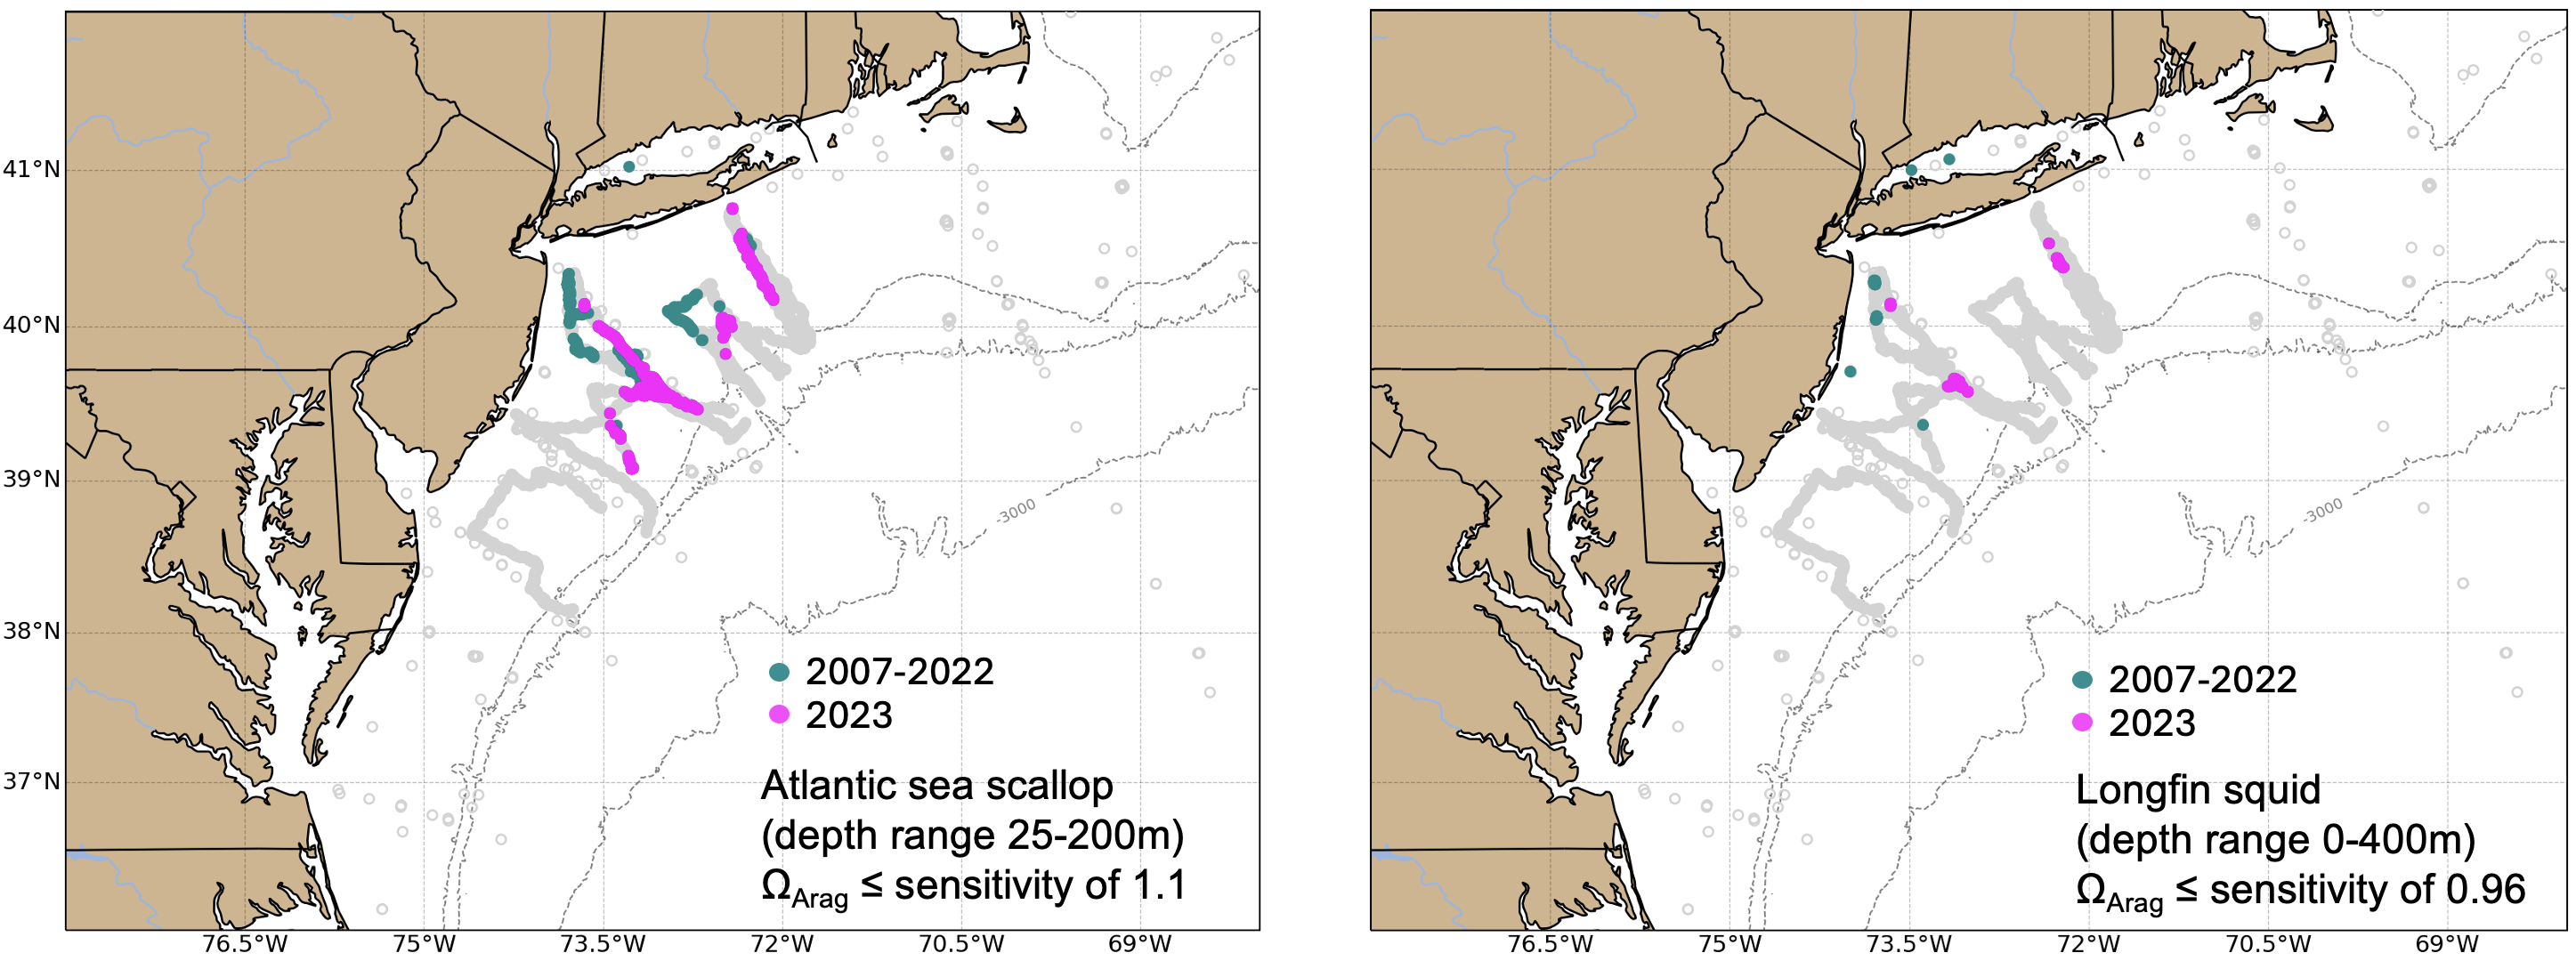
\includegraphics{SOE-NEFMC_files/figure-latex/oa-2023-1} 

}

\caption{Locations where bottom aragonite saturation state ($\Omega_{Arag}$; summer only: June-August) were at or below the laboratory-derived sensitivity level for Atlantic sea scallop (left panel) and longfin squid (right panel) for the time periods 2007-2022 (dark cyan) and 2023 only (magenta). Gray circles indicate locations where bottom $\Omega_{Arag}$ values were above the species specific sensitivity values.}\label{fig:oa-2023}
\end{figure}

Biological and oceanographic processes can affect the amount of oxygen present in the water column. During low oxygen (hypoxic) events, species growth is negatively affected and very low oxygen can result in mortality. The duration and extent of hypoxic events is being monitored, but long-term shelf-wide observations are not yet available. However, \href{https://noaa-edab.github.io/catalog/observation-synthesis.html}{hypoxic events} were detected off the coast of New Jersey in 2023 and were potentially responsible for fish, lobster, and crab \href{https://sebsnjaesnews.rutgers.edu/2023/12/rutgers-scientists-observe-unusual-ocean-conditions-possibly-linked-to-mortality-in-marine-life-off-new-jersey/}{mortalities}.

\hypertarget{drivers-predation}{%
\subparagraph{Drivers: Predation}\label{drivers-predation}}

The abundance and distribution of predators can affect both the productivity and mortality rates on managed stocks. Predators can consume managed species or compete for the same resources resulting in increased natural mortality or productivity, respectively. The northeast shift in \href{https://noaa-edab.github.io/catalog/cetacean-distribution-shifts.html}{highly migratory species} (fig.~\ref{fig:protectedspp-dist-shifts}) indicates a change in the overlap between predators and prey. Since we also observe distribution shifts in both managed and forage species, the effect of changing predator distributions alone is difficult to quantify.

The increase in the \href{https://noaa-edab.github.io/catalog/gray-seal-bycatch.html}{gray seal population} suggests predator populations are increasing in the GOM and GB regions. \href{https://noaa-edab.github.io/catalog/highly-migratory-species-stock-status.html}{Stock status} is mixed for Atlantic Highly Migratory Species (HMS) stocks (including sharks, swordfish, billfish, and tunas) occurring throughout the Northeast U.S shelf. While there are several HMS species considered to be overfished or that have unknown stock status, the population status for some managed Atlantic sharks and tunas is at or above the biomass target (Fig. \ref{fig:hms-stock-status}), suggesting the potential for robust predator populations among these managed species. Stable predator populations suggest stable predation pressure on managed species, but increasing predator populations may reflect increasing predation pressure.

\hypertarget{future-considerations-2}{%
\paragraph{Future Considerations}\label{future-considerations-2}}

The processes that control fish productivity and mortality are dynamic, complex, and the result of the interactions between multiple system drivers. There is a real risk that short-term predictions in assessments and rebuilding plans that assume unchanging underlying conditions will not be as effective, given the observed ecological and environmental process changes documented throughout the report. Assumptions for species' growth, reproduction, and natural mortality should continue to be evaluated for individual species. With observations of system-wide productivity shifts of multiple managed stocks, more research is needed to determine whether regime shifts or ecosystem reorganization are occurring, and how this should be incorporated into management

\hypertarget{other-ocean-uses-offshore-wind}{%
\subsection{Other Ocean Uses: Offshore Wind}\label{other-ocean-uses-offshore-wind}}

\hypertarget{indicators-development-timeline-revenue-in-lease-areas-coastal-community-vulnerability}{%
\subsubsection{Indicators: development timeline, revenue in lease areas, coastal community vulnerability}\label{indicators-development-timeline-revenue-in-lease-areas-coastal-community-vulnerability}}

As of January 2024, 30 offshore \href{https://noaa-edab.github.io/catalog/speed-and-scale-of-offshore-wind-development-in-the-northeast.html}{wind development} projects are proposed for construction over the next decade in the Northeast (timelines and project data for 2024 are based on the Ocean Wind 1 Offshore Wind Farm Final Environmental Impact Statement. Volume II: Appendix F). Offshore wind areas are anticipated to cover more than 2.3 million acres by 2030 in the Greater Atlantic region (Fig. \ref{fig:wind-proposed-dev}). It is anticipated that all states will be able to reach their 2030 offshore wind goals with existing lease areas.

\begin{figure}

{\centering \includegraphics{SOE-NEFMC_files/figure-latex/wind-proposed-dev-1} 

}

\caption{Proposed wind development on the northeast shelf.}\label{fig:wind-proposed-dev}
\end{figure}

Just over 3,300 foundations and more than 12,000 miles of inter-array and offshore export cables are proposed to date. Since first reporting timeline indicators in 2021, construction years by 2030 have become increasingly uncertain with a wide range of estimated construction years being reported for some projects as reflected in the ``Estimated Construction Schedule'' column of Fig. \ref{fig:wind-dev-cumul2} below. The areas affected would be spread out such that it is unlikely that any one particular area would experience full development at one time. Construction of two projects in Southern New England (South Fork Wind and Vineyard Wind 1) during 2023 has affected fisheries managed by the New England Fishery Management Council, while construction activities began for Revolution Wind in early 2024. It is likely that construction will begin on other projects in Southern New England and possibly the New York Bight during 2024 that will further affect regional fisheries.

\begin{figure}

{\centering 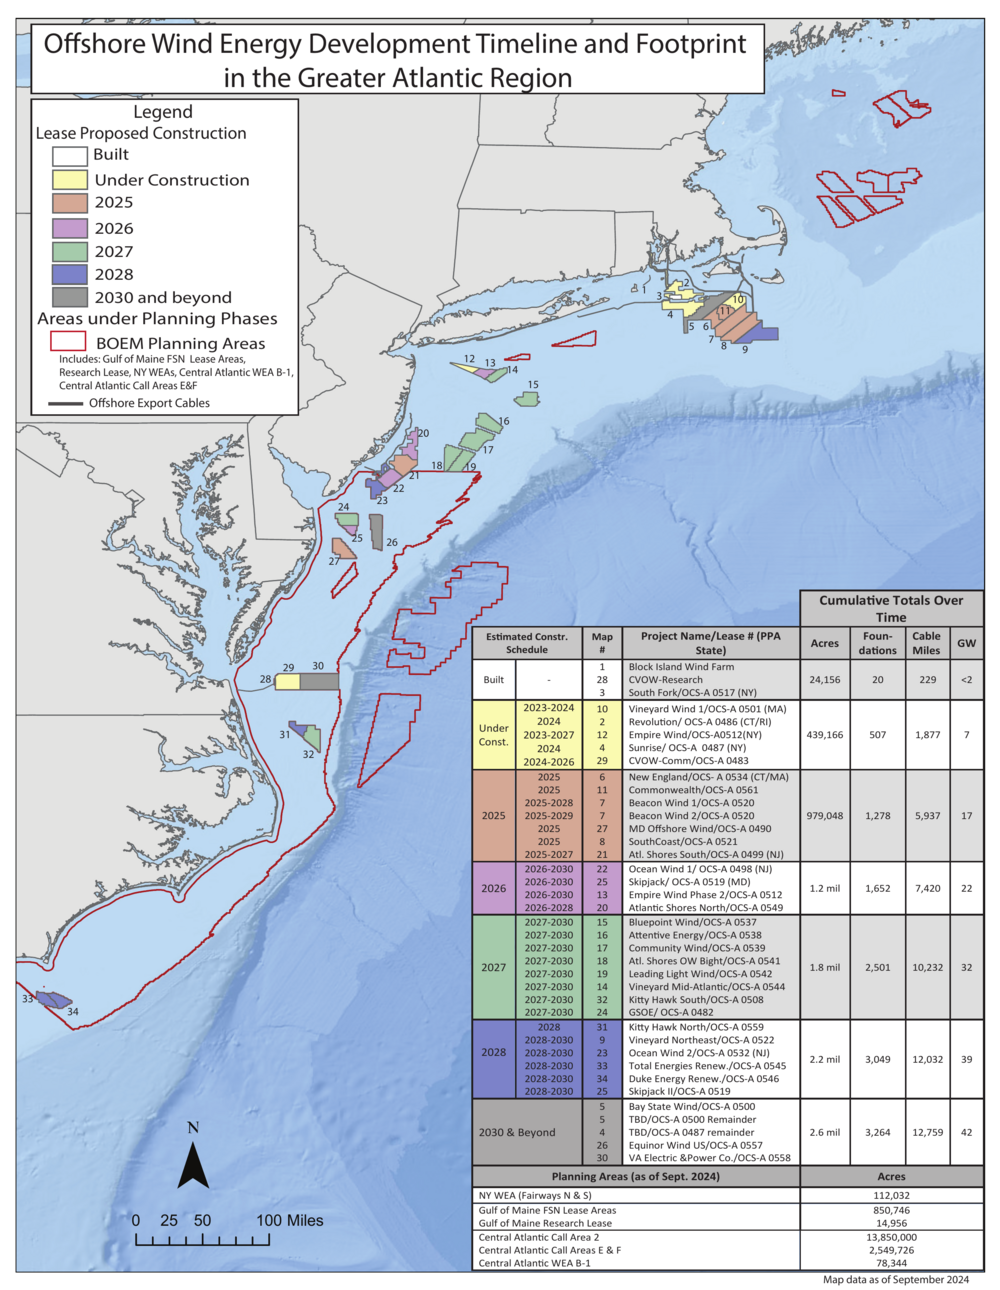
\includegraphics[width=0.9\linewidth]{SOE-NEFMC_files/figure-latex/wind-dev-cumul2-1} 

}

\caption{All Northeast Project areas by year construction ends (each project has 2 year construction period).}\label{fig:wind-dev-cumul2}
\end{figure}
\newpage

Offshore floating wind is expected to be developed in the GOM. Although no commercial wind lease areas have been proposed, BOEM released a draft Wind Energy Area (Fig. \ref{fig:wind-dev-cumul2}) on October 19, 2023, which could be refined into future lease areas. BOEM announced that the final wind energy area and proposed commercial lease area designations for the GOM are expected in quarter one of 2024, with lease sales before 2025. BOEM is also reviewing the state of Maine's application to lease 9,700 acres (15 square miles) for the first floating offshore wind research site in federal waters of the GOM, which could have up to 12 turbines. Leasing for offshore floating wind in the Gulf of Maine will seek to meet the Biden Administration's proposed goal of 15GW of floating offshore wind by 2035 in the U.S.

NEFSC has partnered with the Responsible Ocean Development Alliance (RODA) and the University of Rhode Island to conduct an Integrated Ecosystem Assessment (IEA) of the interactions between offshore wind, fisheries, and the environment in the Gulf of Maine. The IEA report will be similar to the State of the Ecosystem, but fully dedicated to impacts of offshore wind. Data from the IEA will be suitable for inclusion in the environmental impact statements for any projects in the GOM.

Based on federal vessel logbook data, \href{https://noaa-edab.github.io/catalog/fishery-impacts-from-offshore-wind-development.html}{commercial fishery revenue} from trips in the current offshore wind lease areas, the Central Atlantic Final Lease Areas, and the GOM Draft Wind Energy Area (excluding potential secondary areas), represent 3-54\% of the total annual revenue for fisheries managed by the NEFMC from 2008-2022 (Table \ref{table:wea-landings-rev}). Fishing revenue affected by offshore wind lease areas varies over time, but has largely declined over time. Maximum annual revenue for the fisheries with the most overlap with wind lease areas peaked at over \$51 million for the sea scallop fishery, \$4.2 million for monkfish, \$2.2 million for skates, \$724,000 for silver hake, and just over \$1 million for Atlantic herring (Fig. \ref{fig:wea-spp-rev}). The scallop fishery is mainly affected by lease areas in the Mid-Atlantic, as most of the Northern Area scallop fishery is outside of the GOM Draft Wind Energy Area. However, substantially more groundfish landings overlap with the GOM Draft Wind Energy Area, with up to \$15.1 million in annual groundfish revenue caught within potential lease areas. Individual groundfish species are more affected than others, with over 28-53\% of annual revenues for redfish (53\%), pollock (40\%), white hake (34\%) and American plaice (28\%) overlapping with the GOM Draft Wind Energy Area (Table \ref{table:wea-landings-rev}). This potential overlap will decrease once BOEM designates final lease areas for the GOM, which will be substantially smaller than the Draft Wind Energy Area. Future fishery resource overlap with wind leases, especially scallops, may change due to species distribution shifts attributable to climate change and recruitment and larval dispersion pattern changes caused by hydrodynamic flow disruptions from turbine foundations, which could also affect fishery landings/revenue.

\begin{figure}

{\centering \includegraphics{SOE-NEFMC_files/figure-latex/wea-spp-rev-1} 

}

\caption{Fishery revenues from NEFMC managed species in the Wind energy lease areas.}\label{fig:wea-spp-rev}
\end{figure}

\global\setlength{\Oldarrayrulewidth}{\arrayrulewidth}

\global\setlength{\Oldtabcolsep}{\tabcolsep}

\setlength{\tabcolsep}{0pt}

\renewcommand*{\arraystretch}{1}



\providecommand{\ascline}[3]{\noalign{\global\arrayrulewidth #1}\arrayrulecolor[HTML]{#2}\cline{#3}}

\begin{longtable}[c]{|p{2.00in}|p{2.00in}|p{2.00in}}

\caption{Top\ 20\ species\ Landings\ and\ Revenue\ from\ Wind\ Energy\ Areas.\ *A\ very\ small\ amount\ (<500\ lb)\ was\ reported\ landed\ annually\ in\ potential\ offshore\ wind\ energy\ lease\ areas.\ **Landings/revenue\ for\ these\ species\ are\ likely\ underestimated\ due\ to\ limited\ coverage\ of\ these\ fisheries\ in\ existing\ reporting\ requirements\ for\ GARFO-permitted\ vessels.}\label{tab:wea-landings-rev}\\

\ascline{1.5pt}{666666}{1-3}

\multicolumn{1}{>{\raggedright}m{\dimexpr 2in+0\tabcolsep}}{\textcolor[HTML]{000000}{\fontsize{9}{9}\selectfont{NEFMC,\ MAFMC,\ and\ ASMFC\ Managed\ Species}}} & \multicolumn{1}{>{\raggedleft}m{\dimexpr 2in+0\tabcolsep}}{\textcolor[HTML]{000000}{\fontsize{9}{9}\selectfont{Maximum\ Percent\ Total\ Annual\ Regional\ Species\ Landings}}} & \multicolumn{1}{>{\raggedleft}m{\dimexpr 2in+0\tabcolsep}}{\textcolor[HTML]{000000}{\fontsize{9}{9}\selectfont{Maximum\ Percent\ Total\ Annual\ Regional\ Species\ Revenue}}} \\

\ascline{1.5pt}{666666}{1-3}\endfirsthead \caption[]{Top\ 20\ species\ Landings\ and\ Revenue\ from\ Wind\ Energy\ Areas.\ *A\ very\ small\ amount\ (<500\ lb)\ was\ reported\ landed\ annually\ in\ potential\ offshore\ wind\ energy\ lease\ areas.\ **Landings/revenue\ for\ these\ species\ are\ likely\ underestimated\ due\ to\ limited\ coverage\ of\ these\ fisheries\ in\ existing\ reporting\ requirements\ for\ GARFO-permitted\ vessels.}\label{tab:wea-landings-rev}\\

\ascline{1.5pt}{666666}{1-3}

\multicolumn{1}{>{\raggedright}m{\dimexpr 2in+0\tabcolsep}}{\textcolor[HTML]{000000}{\fontsize{9}{9}\selectfont{NEFMC,\ MAFMC,\ and\ ASMFC\ Managed\ Species}}} & \multicolumn{1}{>{\raggedleft}m{\dimexpr 2in+0\tabcolsep}}{\textcolor[HTML]{000000}{\fontsize{9}{9}\selectfont{Maximum\ Percent\ Total\ Annual\ Regional\ Species\ Landings}}} & \multicolumn{1}{>{\raggedleft}m{\dimexpr 2in+0\tabcolsep}}{\textcolor[HTML]{000000}{\fontsize{9}{9}\selectfont{Maximum\ Percent\ Total\ Annual\ Regional\ Species\ Revenue}}} \\

\ascline{1.5pt}{666666}{1-3}\endhead



\multicolumn{1}{>{\raggedright}m{\dimexpr 2in+0\tabcolsep}}{\textcolor[HTML]{000000}{\fontsize{9}{9}\selectfont{Redfish}}} & \multicolumn{1}{>{\raggedleft}m{\dimexpr 2in+0\tabcolsep}}{\textcolor[HTML]{000000}{\fontsize{9}{9}\selectfont{53}}} & \multicolumn{1}{>{\raggedleft}m{\dimexpr 2in+0\tabcolsep}}{\textcolor[HTML]{000000}{\fontsize{9}{9}\selectfont{54}}} \\





\multicolumn{1}{>{\raggedright}m{\dimexpr 2in+0\tabcolsep}}{\textcolor[HTML]{000000}{\fontsize{9}{9}\selectfont{Skates*}}} & \multicolumn{1}{>{\raggedleft}m{\dimexpr 2in+0\tabcolsep}}{\textcolor[HTML]{000000}{\fontsize{9}{9}\selectfont{40}}} & \multicolumn{1}{>{\raggedleft}m{\dimexpr 2in+0\tabcolsep}}{\textcolor[HTML]{000000}{\fontsize{9}{9}\selectfont{51}}} \\





\multicolumn{1}{>{\raggedright}m{\dimexpr 2in+0\tabcolsep}}{\textcolor[HTML]{000000}{\fontsize{9}{9}\selectfont{Pollock}}} & \multicolumn{1}{>{\raggedleft}m{\dimexpr 2in+0\tabcolsep}}{\textcolor[HTML]{000000}{\fontsize{9}{9}\selectfont{43}}} & \multicolumn{1}{>{\raggedleft}m{\dimexpr 2in+0\tabcolsep}}{\textcolor[HTML]{000000}{\fontsize{9}{9}\selectfont{40}}} \\





\multicolumn{1}{>{\raggedright}m{\dimexpr 2in+0\tabcolsep}}{\textcolor[HTML]{000000}{\fontsize{9}{9}\selectfont{White\ hake}}} & \multicolumn{1}{>{\raggedleft}m{\dimexpr 2in+0\tabcolsep}}{\textcolor[HTML]{000000}{\fontsize{9}{9}\selectfont{34}}} & \multicolumn{1}{>{\raggedleft}m{\dimexpr 2in+0\tabcolsep}}{\textcolor[HTML]{000000}{\fontsize{9}{9}\selectfont{34}}} \\





\multicolumn{1}{>{\raggedright}m{\dimexpr 2in+0\tabcolsep}}{\textcolor[HTML]{000000}{\fontsize{9}{9}\selectfont{American\ plaice}}} & \multicolumn{1}{>{\raggedleft}m{\dimexpr 2in+0\tabcolsep}}{\textcolor[HTML]{000000}{\fontsize{9}{9}\selectfont{26}}} & \multicolumn{1}{>{\raggedleft}m{\dimexpr 2in+0\tabcolsep}}{\textcolor[HTML]{000000}{\fontsize{9}{9}\selectfont{28}}} \\





\multicolumn{1}{>{\raggedright}m{\dimexpr 2in+0\tabcolsep}}{\textcolor[HTML]{000000}{\fontsize{9}{9}\selectfont{Atlantic\ halibut}}} & \multicolumn{1}{>{\raggedleft}m{\dimexpr 2in+0\tabcolsep}}{\textcolor[HTML]{000000}{\fontsize{9}{9}\selectfont{23}}} & \multicolumn{1}{>{\raggedleft}m{\dimexpr 2in+0\tabcolsep}}{\textcolor[HTML]{000000}{\fontsize{9}{9}\selectfont{24}}} \\





\multicolumn{1}{>{\raggedright}m{\dimexpr 2in+0\tabcolsep}}{\textcolor[HTML]{000000}{\fontsize{9}{9}\selectfont{Haddock}}} & \multicolumn{1}{>{\raggedleft}m{\dimexpr 2in+0\tabcolsep}}{\textcolor[HTML]{000000}{\fontsize{9}{9}\selectfont{24}}} & \multicolumn{1}{>{\raggedleft}m{\dimexpr 2in+0\tabcolsep}}{\textcolor[HTML]{000000}{\fontsize{9}{9}\selectfont{23}}} \\





\multicolumn{1}{>{\raggedright}m{\dimexpr 2in+0\tabcolsep}}{\textcolor[HTML]{000000}{\fontsize{9}{9}\selectfont{Witch\ flounder}}} & \multicolumn{1}{>{\raggedleft}m{\dimexpr 2in+0\tabcolsep}}{\textcolor[HTML]{000000}{\fontsize{9}{9}\selectfont{25}}} & \multicolumn{1}{>{\raggedleft}m{\dimexpr 2in+0\tabcolsep}}{\textcolor[HTML]{000000}{\fontsize{9}{9}\selectfont{23}}} \\





\multicolumn{1}{>{\raggedright}m{\dimexpr 2in+0\tabcolsep}}{\textcolor[HTML]{000000}{\fontsize{9}{9}\selectfont{Monkfish}}} & \multicolumn{1}{>{\raggedleft}m{\dimexpr 2in+0\tabcolsep}}{\textcolor[HTML]{000000}{\fontsize{9}{9}\selectfont{20}}} & \multicolumn{1}{>{\raggedleft}m{\dimexpr 2in+0\tabcolsep}}{\textcolor[HTML]{000000}{\fontsize{9}{9}\selectfont{20}}} \\





\multicolumn{1}{>{\raggedright}m{\dimexpr 2in+0\tabcolsep}}{\textcolor[HTML]{000000}{\fontsize{9}{9}\selectfont{Atlantic\ surfclam}}} & \multicolumn{1}{>{\raggedleft}m{\dimexpr 2in+0\tabcolsep}}{\textcolor[HTML]{000000}{\fontsize{9}{9}\selectfont{18}}} & \multicolumn{1}{>{\raggedleft}m{\dimexpr 2in+0\tabcolsep}}{\textcolor[HTML]{000000}{\fontsize{9}{9}\selectfont{17}}} \\





\multicolumn{1}{>{\raggedright}m{\dimexpr 2in+0\tabcolsep}}{\textcolor[HTML]{000000}{\fontsize{9}{9}\selectfont{Blueline\ tilefish}}} & \multicolumn{1}{>{\raggedleft}m{\dimexpr 2in+0\tabcolsep}}{\textcolor[HTML]{000000}{\fontsize{9}{9}\selectfont{13}}} & \multicolumn{1}{>{\raggedleft}m{\dimexpr 2in+0\tabcolsep}}{\textcolor[HTML]{000000}{\fontsize{9}{9}\selectfont{16}}} \\





\multicolumn{1}{>{\raggedright}m{\dimexpr 2in+0\tabcolsep}}{\textcolor[HTML]{000000}{\fontsize{9}{9}\selectfont{Yellowtail\ flounder}}} & \multicolumn{1}{>{\raggedleft}m{\dimexpr 2in+0\tabcolsep}}{\textcolor[HTML]{000000}{\fontsize{9}{9}\selectfont{15}}} & \multicolumn{1}{>{\raggedleft}m{\dimexpr 2in+0\tabcolsep}}{\textcolor[HTML]{000000}{\fontsize{9}{9}\selectfont{15}}} \\





\multicolumn{1}{>{\raggedright}m{\dimexpr 2in+0\tabcolsep}}{\textcolor[HTML]{000000}{\fontsize{9}{9}\selectfont{Atlantic\ cod}}} & \multicolumn{1}{>{\raggedleft}m{\dimexpr 2in+0\tabcolsep}}{\textcolor[HTML]{000000}{\fontsize{9}{9}\selectfont{15}}} & \multicolumn{1}{>{\raggedleft}m{\dimexpr 2in+0\tabcolsep}}{\textcolor[HTML]{000000}{\fontsize{9}{9}\selectfont{15}}} \\





\multicolumn{1}{>{\raggedright}m{\dimexpr 2in+0\tabcolsep}}{\textcolor[HTML]{000000}{\fontsize{9}{9}\selectfont{Black\ sea\ bass}}} & \multicolumn{1}{>{\raggedleft}m{\dimexpr 2in+0\tabcolsep}}{\textcolor[HTML]{000000}{\fontsize{9}{9}\selectfont{10}}} & \multicolumn{1}{>{\raggedleft}m{\dimexpr 2in+0\tabcolsep}}{\textcolor[HTML]{000000}{\fontsize{9}{9}\selectfont{10}}} \\





\multicolumn{1}{>{\raggedright}m{\dimexpr 2in+0\tabcolsep}}{\textcolor[HTML]{000000}{\fontsize{9}{9}\selectfont{Atlantic\ sea\ scallop}}} & \multicolumn{1}{>{\raggedleft}m{\dimexpr 2in+0\tabcolsep}}{\textcolor[HTML]{000000}{\fontsize{9}{9}\selectfont{10}}} & \multicolumn{1}{>{\raggedleft}m{\dimexpr 2in+0\tabcolsep}}{\textcolor[HTML]{000000}{\fontsize{9}{9}\selectfont{9}}} \\





\multicolumn{1}{>{\raggedright}m{\dimexpr 2in+0\tabcolsep}}{\textcolor[HTML]{000000}{\fontsize{9}{9}\selectfont{Scup}}} & \multicolumn{1}{>{\raggedleft}m{\dimexpr 2in+0\tabcolsep}}{\textcolor[HTML]{000000}{\fontsize{9}{9}\selectfont{8}}} & \multicolumn{1}{>{\raggedleft}m{\dimexpr 2in+0\tabcolsep}}{\textcolor[HTML]{000000}{\fontsize{9}{9}\selectfont{9}}} \\





\multicolumn{1}{>{\raggedright}m{\dimexpr 2in+0\tabcolsep}}{\textcolor[HTML]{000000}{\fontsize{9}{9}\selectfont{Atlantic\ mackerel}}} & \multicolumn{1}{>{\raggedleft}m{\dimexpr 2in+0\tabcolsep}}{\textcolor[HTML]{000000}{\fontsize{9}{9}\selectfont{8}}} & \multicolumn{1}{>{\raggedleft}m{\dimexpr 2in+0\tabcolsep}}{\textcolor[HTML]{000000}{\fontsize{9}{9}\selectfont{8}}} \\





\multicolumn{1}{>{\raggedright}m{\dimexpr 2in+0\tabcolsep}}{\textcolor[HTML]{000000}{\fontsize{9}{9}\selectfont{Longfin\ squid}}} & \multicolumn{1}{>{\raggedleft}m{\dimexpr 2in+0\tabcolsep}}{\textcolor[HTML]{000000}{\fontsize{9}{9}\selectfont{8}}} & \multicolumn{1}{>{\raggedleft}m{\dimexpr 2in+0\tabcolsep}}{\textcolor[HTML]{000000}{\fontsize{9}{9}\selectfont{8}}} \\





\multicolumn{1}{>{\raggedright}m{\dimexpr 2in+0\tabcolsep}}{\textcolor[HTML]{000000}{\fontsize{9}{9}\selectfont{Red\ hake}}} & \multicolumn{1}{>{\raggedleft}m{\dimexpr 2in+0\tabcolsep}}{\textcolor[HTML]{000000}{\fontsize{9}{9}\selectfont{11}}} & \multicolumn{1}{>{\raggedleft}m{\dimexpr 2in+0\tabcolsep}}{\textcolor[HTML]{000000}{\fontsize{9}{9}\selectfont{8}}} \\





\multicolumn{1}{>{\raggedright}m{\dimexpr 2in+0\tabcolsep}}{\textcolor[HTML]{000000}{\fontsize{9}{9}\selectfont{Silver\ hake}}} & \multicolumn{1}{>{\raggedleft}m{\dimexpr 2in+0\tabcolsep}}{\textcolor[HTML]{000000}{\fontsize{9}{9}\selectfont{9}}} & \multicolumn{1}{>{\raggedleft}m{\dimexpr 2in+0\tabcolsep}}{\textcolor[HTML]{000000}{\fontsize{9}{9}\selectfont{7}}} \\

\ascline{1.5pt}{666666}{1-3}



\end{longtable}



\arrayrulecolor[HTML]{000000}

\global\setlength{\arrayrulewidth}{\Oldarrayrulewidth}

\global\setlength{\tabcolsep}{\Oldtabcolsep}

\renewcommand*{\arraystretch}{1}

Equity and environmental justice (EJ) are priority concerns with offshore wind development and fisheries impacts in the Northeast, and the impacts of offshore wind development are expected to differentially \href{https://noaa-edab.github.io/catalog/community-port-landings-and-revenue-from-wind-energy-areas-weas.html}{impact specific coastal communities}. Additionally, impacts of offshore wind development may unevenly affect individual operators, with some permit holders deriving a much higher proportion of revenue from wind areas than the port-based mean.

\begin{figure}

\includegraphics{SOE-NEFMC_files/figure-latex/wea-port-rev-1} \hfill{}

\caption{Percent of port fisheries revenue from Wind Energy Areas (WEA) in descending order from most to least port fisheries revenue from WEA. EJ = Environmental Justice.}\label{fig:wea-port-rev}
\end{figure}

For example, Little Compton, RI had a minimum of 17\% and maximum of 32\% overlap of wind energy revenue to the total port revenue between 2008-2022 (Fig. \ref{fig:wea-port-rev}). BOEM reports that cumulative offshore wind development (if all proposed projects are developed) could have moderate impacts on low-income members of environmental justice communities who work in the commercial fishing and for-hire fishing industry due to disruptions to fish populations, restrictions on navigation and increased vessel traffic as well as existing vulnerabilities of low-income workers to economic impacts.

Top fishing communities with high \href{https://noaa-edab.github.io/catalog/engagement-reliance-and-environmental-justice-in-top-fishing-communities.html}{environmental justice concerns} such as New Bedford, MA, New London, CT should be considered in decision making to reduce the social and economic impacts and aid in the resilience and adaptive capacity of underserved communities. These two ports are also undergoing significant changes to support offshore wind development port infrastructure needs. Environmental justice concerns also highlight communities where further resources are needed to reach underserved and underrepresented groups and create opportunities for, and directly involve, these groups in the decision-making process.

\begin{figure}

\includegraphics{SOE-NEFMC_files/figure-latex/wind-rev-MAB-NEFMC-1} \hfill{}

\caption{Percent of Mid-Atlantic port revenue with majority NEFMC landings from Wind Energy Areas (WEA) in descending order from most to least port fisheries revenue from WEA. EJ = Environmental Justice.}\label{fig:wind-rev-MAB-NEFMC}
\end{figure}

\hypertarget{implications-6}{%
\subsubsection{Implications}\label{implications-6}}

Current plans for rapid buildout of offshore wind in a patchwork of areas spreads the impacts differentially throughout the region (Fig. \ref{fig:wind-dev-cumul2}).

Up to 12\% of total average revenue for major New England commercial species in lease areas could be forgone, or reduced, and associated effort displaced if all sites are developed. Displaced fishing effort can alter historic fishing areas, timing, and methods, which can in turn change habitat, species (managed and protected), and fleet interactions. Several factors, including fishery regulations, fishery availability, and user conflicts affect where, when, and how fishing effort may be displaced, along with impacts to and responses of affected fish species.

Planned development \href{https://noaa-edab.github.io/catalog/right-whale-abundance.html}{overlaps NARW} mother and calf migration corridors and a significant foraging habitat that is used throughout the year (Fig. \ref{fig:whales-wind}). Turbine presence and extraction of energy from the system could alter local oceanography and may affect right whale prey availability. For example, persistent foraging hotspots of right whales and seabirds overlap on Nantucket Shoals, where unique hydrography aggregates enhanced prey densities. Wind leases (OCS-A 0521 and OCS-A 0522) currently intersect these hotspots on the southwestern corner of Nantucket Shoals and a prominent tidal front associated with invertebrate prey swarms important to seabirds and possibly right whales. Proposed wind development areas also bring increased vessel strike risk from construction and operation vessels. In addition, there are a number of potential impacts to whales from pile driving and operational noise such as displacement, increased levels of communication masking, and elevated stress hormones.

Proposed wind development areas interact with the region's federal scientific surveys. Scientific surveys are impacted by offshore wind in four ways:

\begin{enumerate}
\def\labelenumi{\arabic{enumi}.}
\tightlist
\item
  Exclusion of NOAA Fisheries' sampling platforms from the wind development area due to operational and safety limitations
\item
  Impacts on the random-stratified statistical design that is the basis for scientific assessments, advice, and analyses;
\item
  Alteration of benthic and pelagic habitats, and airspace in and around the wind energy development, requiring new designs and methods to sample new habitats
\item
  Reduced sampling productivity through navigation impacts of wind energy infrastructure on aerial and vessel survey operations
\end{enumerate}

Increased vessel transit between stations may decrease data collections that are already limited by annual days-at-sea day allocations. The total survey area overlap ranges from 1-70\% for all Greater Atlantic federal surveys. The Gulf of Maine Cooperative Research Bottom Longline Survey (41\%) and the Shrimp Survey (70\%) have the largest percent overlap with the draft Gulf of Maine Wind Energy Areas. The remaining surveys range from 1-16\% overlap. Individual survey strata have significant interaction with wind, including the sea scallop survey (up to 96\% of individual strata) and the bottom trawl survey (BTS, up to 60\% strata overlap). Additionally, up to 50\% of the southern New England North Atlantic right whale survey's area overlaps with proposed project areas and A region-wide survey mitigation program is underway

The increase of offshore wind development can have both positive (e.g., employment opportunities) and negative (e.g., space-use conflicts) sociocultural effects. Continued increase in coastal development and gentrification pressure has resulted in loss of fishing infrastructure space within ports. Understanding these existing pressures can help avoid and mitigate negative impacts to our shore support industry and communities dependent on fishing. Some of the communities with the highest fisheries revenue overlap with offshore wind development areas that are also vulnerable to gentrification pressure are Point Judith and Newport, RI, New Bedford, MA, Port Clyde and Portland, ME.

\begin{figure}

{\centering \includegraphics[width=0.6\linewidth]{SOE-NEFMC_files/figure-latex/whales-wind-1} 

}

\caption{Northern Right Whale persistent hotspots and Wind Energy Areas.}\label{fig:whales-wind}
\end{figure}
\newpage

\hypertarget{current-state-2023-observations}{%
\subsection{Current state: 2023 Observations}\label{current-state-2023-observations}}

Multiple \href{https://noaa-edab.github.io/catalog/observation-synthesis.html}{anomalous conditions} and extreme events were observed in 2023 that could have brief local effects and/or widespread long-term ecosystem, fishery and management implications. This section intends to provide a record of these observations, the implications they may have for other ecosystem processes, and a reflection on how they fit into our understanding of the ecosystem. Many of these observations are being actively studied but should be noted and considered in future analyses and management decisions.

Globally, 2023 was the warmest year on record with record high sea surface temperatures in the North Atlantic. In contrast, Northeast U.S. shelf surface temperatures were more variable, with near record highs in winter and near average conditions in other seasons.

\hypertarget{regionalcoastal-phenomena}{%
\subsubsection{Regional/Coastal Phenomena}\label{regionalcoastal-phenomena}}

There was a documented \href{https://noaa-edab.github.io/catalog/observation-synthesis.html}{die-off of scallops} in the Mid-Atlantic Elephant Trunk regions between the 2022 and 2023 surveys. In 2022, Elephant Trunk experienced \href{https://noaa-edab.github.io/catalog/thermal-habitat-persistence.html}{stressful temperatures} for scallops (17 - 19 ℃) for an average of 30 days, (Fig. \ref{fig:scallop-thermal-2022}) but ongoing research is being conducted to identify contributing factors. A fish and shellfish mortality event was observed in coastal New Jersey linked to \href{https://noaa-edab.github.io/catalog/ocean-acidification-and-other-stressors.html}{hypoxia and ocean acidification} (Fig. \ref{fig:hypoxia-2023}).

\begin{figure}

{\centering \includegraphics[width=0.6\linewidth]{SOE-NEFMC_files/figure-latex/scallop-thermal-2022-1} 

}

\caption{The number of days where bottom temperature was between 17 and 19 ℃ in each GLORYS grid cell for 2022. The gray lines show the sea scallop estimation areas, with the Elephant Trunk region highlighted in black lines.}\label{fig:scallop-thermal-2022}
\end{figure}
\begin{figure}

{\centering \includegraphics[width=0.6\linewidth]{SOE-NEFMC_files/figure-latex/hypoxia-2023-1} 

}

\caption{Mission tracks of three gliders (left) deployed off the coast of New Jersey in August and September of 2023. Locations of hypoxic levels of dissolved oxygen (magenta; < 3 mg/liter) and low aragonite saturation state (cyan; < 1) measured along the glider mission tracks and locations of reported fish, lobster, and/or crab mortalities (red X).}\label{fig:hypoxia-2023}
\end{figure}

Summer \href{https://noaa-edab.github.io/catalog/bottom-temperature---seasonal-anomaly.html}{bottom temperatures} in the Gulf of Maine were the warmest on record (since 1959) resulting in the second largest \href{https://noaa-edab.github.io/catalog/marine-heatwaves---bottom.html}{bottom marine heatwave}. The heatwave started in February, peaked in May and likely continued beyond August (pending data update). 2023 \href{https://noaa-edab.github.io/catalog/thermal-habitat-persistence.html}{bottom temperature} exceeded the 15oC threshold for up to 59 days along the shelf break.

A wide-spread, long-duration \href{https://noaa-edab.github.io/catalog/observation-synthesis.html}{phytoplankton bloom} of the dinoflagellate Tripos muelleri was observed in the GOM and generated \href{https://noaa-edab.github.io/catalog/chlorophyll-and-primary-production.html}{chlorophyll concentrations} up to ten times greater than average (a record high since 1998) from March to August (Fig. \ref{fig:gom-bloom-2023}). The bloom severely reduced water clarity, impacting harpoon fishing and likely affecting visual predators. Despite Tripos being a similar size to typical large phytoplankton (diatoms), this extra production was not grazed nor did it sink to the bottom. The specific drivers of the bloom and implications to the food web are still under investigation.

\begin{figure}

{\centering \includegraphics[width=0.6\linewidth]{SOE-NEFMC_files/figure-latex/gom-bloom-2023-1} 

}

\caption{Map of Chlorophyll anomaly ratio in 2023 during a large bloom event.}\label{fig:gom-bloom-2023}
\end{figure}

In Chesapeake Bay, \href{https://noaa-edab.github.io/catalog/chesapeake-bay-2023-synthesis.html}{hypoxia conditions} were the lowest on record (since 1995), creating more suitable habitat for multiple fin fish and benthic species. Cooler \href{https://noaa-edab.github.io/catalog/chesapeake-bay-seasonal-sea-surface-temperature-anomaly.html}{Chesapeake Bay water temperatures} paired with low hypoxia in the summer suggest conditions that season were favorable for striped bass. Cooler summer temperatures also support juvenile summer flounder growth. However, warmer winter and spring water temperatures in the Chesapeake Bay, along with other environmental factors (such as low flow), may have played a role in low production of juvenile striped bass in 2023.

Higher-than-average \href{https://noaa-edab.github.io/catalog/chesapeake-bay-salinity.html}{salinity} across the Bay was likely driven by low precipitation and increased the area of available habitat for species such as croaker, spot, menhaden, and red drum, while restricting habitat area for invasive blue catfish.

\hypertarget{shelf-wide-phenomena}{%
\subsubsection{Shelf-wide Phenomena}\label{shelf-wide-phenomena}}

The \href{https://noaa-edab.github.io/catalog/gulf-stream-index.html}{Gulf Stream} was highly variable in 2023, with northward shifts intermittently throughout the year and a more notable prolonged shift north along the continental shelf break in the southern Mid-Atlantic in the fall {[}Fig .\ref{fig:gulf-stream-2023}{]}. This shift severely constricted the Slope Sea (the waters between the Gulf Stream and continental shelf), inhibited warm core ring formation and interactions, resulted in unusually warm and salty surface waters, and strong northeastward currents in the southern Mid-Atlantic. Intermittent warm waters like this can be threats to temperature sensitive species, especially species at the southern end of their range or are not mobile (e.g.~scallops), while also providing suitable habitat for more southern species.

\begin{figure}

{\centering \includegraphics[width=0.6\linewidth]{SOE-NEFMC_files/figure-latex/gulf-stream-2023-1} 

}

\caption{Map of sea surface temeprature (color scale) in October, 2023. The dark blue line shows the long-term mean Gulf Steam position.}\label{fig:gulf-stream-2023}
\end{figure}

While the total number of \href{https://noaa-edab.github.io/catalog/warm-core-rings.html}{warm core rings} in 2023 (18) was below the decadal average (31), there were a few notable events. A large early season ring pulled continental shelf water into the Slope Sea. Events like these can create biological hotspots, aggregating multiple species in small areas, increasing bycatch risks, and marine mammal shipstrike risks. In spring 2023, concentrations of \href{https://noaa-edab.github.io/catalog/persistent-annual-hotspots.html?q=hotspo\#persistent-annual-hotspots}{North Atlantic right whales}, humpback whales, basking sharks, and other large baleen whales were observed feeding near the edge of warm core rings near the shelf break.

Multiple fall 2023 tropical and coastal storms caused several flash flood events, above average coastal water levels, strong winds and high rainfall totals throughout the Northeast. These storms may be related to the shift from 2020-2022 La Niña conditions to strong El Niño conditions in late spring 2023. El Niño winters are associated with more frequent East Coast storms, which can result in increased risk of coastal flooding, increased freshwater runoff into the coastal ocean, and delayed spring transition from a well mixed water column to stratified. In estuaries, increased freshwater flow decreases salinity, reduces the amount of suitable habitat for juvenile marine fish, and is related to increased hypoxia (low oxygen). However, precipitation is not uniform throughout the Northeast U.S., and \href{https://noaa-edab.github.io/catalog/chesapeake-bay-salinity.html}{Chesapeake Bay 2023 conditions} did not align with El Niño expectations. The current El Niño is expected to weaken by spring 2024.

\hypertarget{contributors}{%
\section{Contributors}\label{contributors}}

\textbf{Editors} (NOAA NMFS Northeast Fisheries Science Center, NEFSC): Joseph Caracappa, Sarah Gaichas, Brandon Beltz, Geret DePiper, Kimberly Hyde, Scott Large, Laurel Smith.

\textbf{Contributors} (NEFSC unless otherwise noted): Kimberly Bastille, Aaron Beaver (Anchor QEA), Andy Beet, Ruth Boettcher (Virginia Department of Game and Inland Fisheries), Mandy Bromilow (NOAA Chesapeake Bay Office), Joseph Caracappa, Zhuomin Chen (University of Connecticut), Doug Christel (GARFO), Patricia Clay, Lisa Colburn, Jennifer Cudney (NMFS Atlantic HMS Management Division), Tobey Curtis (NMFS Atlantic HMS Management Division), Geret DePiper, Dan Dorfman (NOAA-NOS-NCCOS), Hubert du Pontavice, Emily Farr (NMFS Office of Habitat Conservation), Michael Fogarty, Paula Fratantoni, Kevin Friedland, Marjy Friedrichs (VIMS), Sarah Gaichas, Ben Galuardi (GARFO), Avijit Gangopadhyay (School for Marine Science and Technology, University of Massachusetts Dartmouth), James Gartland (Virginia Institute of Marine Science), Glen Gawarkiewicz (Woods Hole Oceanographic Institution), Sean Hardison, Dvora Hart, Kimberly Hyde, John Kocik, Steve Kress (National Audubon Society's Seabird Restoration Program), Young-Oh Kwon (Woods Hole Oceanographic Institution), Andrew Lipsky, Sean Lucey, Don Lyons (National Audubon Society's Seabird Restoration Program), Chris Melrose, Shannon Meseck, Ryan Morse, Brandon Muffley (MAFMC), Kimberly Murray, Chris Orphanides, Richard Pace, Tom Parham (Maryland DNR), CJ Pellerin (NOAA Chesapeake Bay Office), Charles Perretti, Grace Roskar (NMFS Office of Habitat Conservation), Grace Saba (Rutgers), Vincent Saba, Sarah Salois, Chris Schillaci (GARFO), Dave Secor (CBL), Angela Silva, Adrienne Silver (UMass/SMAST), Emily Slesinger (Rutgers University), Laurel Smith, Talya tenBrink (GARFO), Abigail Tyrell, Bruce Vogt (NOAA Chesapeake Bay Office), Ron Vogel (University of Maryland Cooperative Institute of Satellite Earth System Studies and NOAA/NESDIS Center for Satellite Applications and Research), John Walden, Harvey Walsh, Changhua Weng, Timothy White (Environmental Studies Program, BOEM), Mark Wuenschel.

\newpage

\hypertarget{document-orientation}{%
\section{Document Orientation}\label{document-orientation}}

The figure format is illustrated in Fig \ref{fig:docformat}a. Trend lines are shown when the slope is significantly different from 0 at the p \textless{} 0.05 level. An orange line signifies an overall positive trend, and purple signifies a negative trend. To minimize bias introduced by small sample size, no trend is fit for \textless{} 30 year time series. Dashed lines represent mean values of time series unless the indicator is an anomaly, in which case the dashed line is equal to 0. Shaded regions indicate the past ten years. If there are no new data for 2020, the shaded region will still cover this time period. The spatial scale of indicators is either coastwide, New England states (Connecticut, Rhode Island, Massachusetts, New Hampshire, and Maine), or at one of the two Ecosystem Production Units (EPUs, Fig. \ref{fig:docformat}b) levels in the region, Georges Bank (GB) or Gulf of Maine (GOM).

\begin{figure}

{\centering \includegraphics{SOE-NEFMC_files/figure-latex/docformat-1} 

}

\caption{Document orientation. a. Key to figures. b.The Northeast Large Marine Ecosystem.}\label{fig:docformat}
\end{figure}

Fish and invertebrates are aggregated into similar \href{https://noaa-edab.github.io/catalog/feeding-guilds-by-management-bodies.html}{feeding guild categories} (Table \ref{tab:species-groupings}) to evaluate ecosystem level trends in predators and prey.

\global\setlength{\Oldarrayrulewidth}{\arrayrulewidth}

\global\setlength{\Oldtabcolsep}{\tabcolsep}

\setlength{\tabcolsep}{0pt}

\renewcommand*{\arraystretch}{1.5}



\providecommand{\ascline}[3]{\noalign{\global\arrayrulewidth #1}\arrayrulecolor[HTML]{#2}\cline{#3}}

\begin{longtable}[c]{|p{1.00in}|p{1.00in}|p{1.00in}|p{1.00in}|p{3.00in}}

\caption{Feeding\ guilds\ and\ management\ bodies.}\label{tab:species-groupings}\\

\ascline{1.5pt}{666666}{1-5}

\multicolumn{1}{>{\raggedright}m{\dimexpr 1in+0\tabcolsep}}{\textcolor[HTML]{000000}{\fontsize{8}{8}\selectfont{Guild}}} & \multicolumn{1}{>{\raggedright}m{\dimexpr 1in+0\tabcolsep}}{\textcolor[HTML]{000000}{\fontsize{8}{8}\selectfont{MAFMC}}} & \multicolumn{1}{>{\raggedright}m{\dimexpr 1in+0\tabcolsep}}{\textcolor[HTML]{000000}{\fontsize{8}{8}\selectfont{Joint}}} & \multicolumn{1}{>{\raggedright}m{\dimexpr 1in+0\tabcolsep}}{\textcolor[HTML]{000000}{\fontsize{8}{8}\selectfont{NEFMC}}} & \multicolumn{1}{>{\raggedright}m{\dimexpr 3in+0\tabcolsep}}{\textcolor[HTML]{000000}{\fontsize{8}{8}\selectfont{State\ or\ Other}}} \\

\ascline{1.5pt}{666666}{1-5}\endfirsthead \caption[]{Feeding\ guilds\ and\ management\ bodies.}\label{tab:species-groupings}\\

\ascline{1.5pt}{666666}{1-5}

\multicolumn{1}{>{\raggedright}m{\dimexpr 1in+0\tabcolsep}}{\textcolor[HTML]{000000}{\fontsize{8}{8}\selectfont{Guild}}} & \multicolumn{1}{>{\raggedright}m{\dimexpr 1in+0\tabcolsep}}{\textcolor[HTML]{000000}{\fontsize{8}{8}\selectfont{MAFMC}}} & \multicolumn{1}{>{\raggedright}m{\dimexpr 1in+0\tabcolsep}}{\textcolor[HTML]{000000}{\fontsize{8}{8}\selectfont{Joint}}} & \multicolumn{1}{>{\raggedright}m{\dimexpr 1in+0\tabcolsep}}{\textcolor[HTML]{000000}{\fontsize{8}{8}\selectfont{NEFMC}}} & \multicolumn{1}{>{\raggedright}m{\dimexpr 3in+0\tabcolsep}}{\textcolor[HTML]{000000}{\fontsize{8}{8}\selectfont{State\ or\ Other}}} \\

\ascline{1.5pt}{666666}{1-5}\endhead



\multicolumn{1}{>{\raggedright}m{\dimexpr 1in+0\tabcolsep}}{\textcolor[HTML]{000000}{\fontsize{8}{8}\selectfont{Apex\ Predator}}} & \multicolumn{1}{>{\raggedright}m{\dimexpr 1in+0\tabcolsep}}{\textcolor[HTML]{000000}{\fontsize{8}{8}\selectfont{}}} & \multicolumn{1}{>{\raggedright}m{\dimexpr 1in+0\tabcolsep}}{\textcolor[HTML]{000000}{\fontsize{8}{8}\selectfont{}}} & \multicolumn{1}{>{\raggedright}m{\dimexpr 1in+0\tabcolsep}}{\textcolor[HTML]{000000}{\fontsize{8}{8}\selectfont{}}} & \multicolumn{1}{>{\raggedright}m{\dimexpr 3in+0\tabcolsep}}{\textcolor[HTML]{000000}{\fontsize{8}{8}\selectfont{shark\ uncl,\ swordfish,\ yellowfin\ tuna,\ bluefin\ tuna}}} \\





\multicolumn{1}{>{\raggedright}m{\dimexpr 1in+0\tabcolsep}}{\textcolor[HTML]{000000}{\fontsize{8}{8}\selectfont{Piscivore}}} & \multicolumn{1}{>{\raggedright}m{\dimexpr 1in+0\tabcolsep}}{\textcolor[HTML]{000000}{\fontsize{8}{8}\selectfont{summer\ flounder,\ bluefish,\ northern\ shortfin\ squid,\ longfin\ squid}}} & \multicolumn{1}{>{\raggedright}m{\dimexpr 1in+0\tabcolsep}}{\textcolor[HTML]{000000}{\fontsize{8}{8}\selectfont{spiny\ dogfish,\ goosefish}}} & \multicolumn{1}{>{\raggedright}m{\dimexpr 1in+0\tabcolsep}}{\textcolor[HTML]{000000}{\fontsize{8}{8}\selectfont{winter\ skate,\ clearnose\ skate,\ thorny\ skate,\ offshore\ hake,\ silver\ hake,\ atlantic\ cod,\ pollock,\ white\ hake,\ red\ hake,\ atlantic\ halibut,\ acadian\ redfish}}} & \multicolumn{1}{>{\raggedright}m{\dimexpr 3in+0\tabcolsep}}{\textcolor[HTML]{000000}{\fontsize{8}{8}\selectfont{sea\ lamprey,\ sandbar\ shark,\ atlantic\ angel\ shark,\ atlantic\ torpedo,\ conger\ eel,\ spotted\ hake,\ cusk,\ fourspot\ flounder,\ windowpane,\ john\ dory,\ atlantic\ cutlassfish,\ blue\ runner,\ striped\ bass,\ weakfish,\ sea\ raven,\ northern\ stargazer,\ banded\ rudderfish,\ atlantic\ sharpnose\ shark,\ inshore\ lizardfish,\ atlantic\ brief\ squid,\ northern\ sennet,\ king\ mackerel,\ spanish\ mackerel}}} \\





\multicolumn{1}{>{\raggedright}m{\dimexpr 1in+0\tabcolsep}}{\textcolor[HTML]{000000}{\fontsize{8}{8}\selectfont{Planktivore}}} & \multicolumn{1}{>{\raggedright}m{\dimexpr 1in+0\tabcolsep}}{\textcolor[HTML]{000000}{\fontsize{8}{8}\selectfont{atlantic\ mackerel,\ butterfish}}} & \multicolumn{1}{>{\raggedright}m{\dimexpr 1in+0\tabcolsep}}{\textcolor[HTML]{000000}{\fontsize{8}{8}\selectfont{}}} & \multicolumn{1}{>{\raggedright}m{\dimexpr 1in+0\tabcolsep}}{\textcolor[HTML]{000000}{\fontsize{8}{8}\selectfont{atlantic\ herring}}} & \multicolumn{1}{>{\raggedright}m{\dimexpr 3in+0\tabcolsep}}{\textcolor[HTML]{000000}{\fontsize{8}{8}\selectfont{harvestfishes,\ smelts,\ round\ herring,\ alewife,\ blueback\ herring,\ american\ shad,\ menhaden,\ bay\ anchovy,\ striped\ anchovy,\ rainbow\ smelt,\ atlantic\ argentine,\ slender\ snipe\ eel,\ atlantic\ silverside,\ northern\ pipefish,\ chub\ mackerel,\ atlantic\ moonfish,\ lookdown,\ blackbelly\ rosefish,\ lumpfish,\ northern\ sand\ lance,\ atlantic\ saury,\ mackerel\ scad,\ bigeye\ scad,\ round\ scad,\ rough\ scad,\ silver\ rag,\ weitzmans\ pearlsides,\ atlantic\ soft\ pout,\ sevenspine\ bay\ shrimp,\ pink\ glass\ shrimp,\ polar\ lebbeid,\ friendly\ blade\ shrimp,\ bristled\ longbeak,\ aesop\ shrimp,\ norwegian\ shrimp,\ northern\ shrimp,\ brown\ rock\ shrimp,\ atlantic\ thread\ herring,\ spanish\ sardine,\ atlantic\ bumper,\ harvestfish,\ striated\ argentine,\ silver\ anchovy}}} \\





\multicolumn{1}{>{\raggedright}m{\dimexpr 1in+0\tabcolsep}}{\textcolor[HTML]{000000}{\fontsize{8}{8}\selectfont{Benthivore}}} & \multicolumn{1}{>{\raggedright}m{\dimexpr 1in+0\tabcolsep}}{\textcolor[HTML]{000000}{\fontsize{8}{8}\selectfont{black\ sea\ bass,\ scup,\ tilefish}}} & \multicolumn{1}{>{\raggedright}m{\dimexpr 1in+0\tabcolsep}}{\textcolor[HTML]{000000}{\fontsize{8}{8}\selectfont{}}} & \multicolumn{1}{>{\raggedright}m{\dimexpr 1in+0\tabcolsep}}{\textcolor[HTML]{000000}{\fontsize{8}{8}\selectfont{barndoor\ skate,\ rosette\ skate,\ little\ skate,\ smooth\ skate,\ haddock,\ american\ plaice,\ yellowtail\ flounder,\ winter\ flounder,\ witch\ flounder,\ ocean\ pout,\ crab,red\ deepsea}}} & \multicolumn{1}{>{\raggedright}m{\dimexpr 3in+0\tabcolsep}}{\textcolor[HTML]{000000}{\fontsize{8}{8}\selectfont{crab,unc,\ hagfish,\ porgy,red,\ sea\ bass,nk,\ atlantic\ hagfish,\ roughtail\ stingray,\ smooth\ dogfish,\ chain\ dogfish,\ bluntnose\ stingray,\ bullnose\ ray,\ southern\ stingray,\ longfin\ hake,\ fourbeard\ rockling,\ marlin-spike,\ gulf\ stream\ flounder,\ longspine\ snipefish,\ blackmouth\ bass,\ threespine\ stickleback,\ smallmouth\ flounder,\ hogchoker,\ bigeye,\ atlantic\ croaker,\ pigfish,\ northern\ kingfish,\ silver\ perch,\ spot,\ deepbody\ boarfish,\ sculpin\ uncl,\ moustache\ sculpin,\ longhorn\ sculpin,\ alligatorfish,\ grubby,\ atlantic\ seasnail,\ northern\ searobin,\ striped\ searobin,\ armored\ searobin,\ cunner,\ tautog,\ snakeblenny,\ daubed\ shanny,\ radiated\ shanny,\ red\ goatfish,\ striped\ cusk-eel,\ wolf\ eelpout,\ wrymouth,\ atlantic\ wolffish,\ fawn\ cusk-eel,\ northern\ puffer,\ striped\ burrfish,\ planehead\ filefish,\ gray\ triggerfish,\ shortnose\ greeneye,\ beardfish,\ cownose\ ray,\ american\ lobster,\ cancer\ crab\ uncl,\ jonah\ crab,\ atlantic\ rock\ crab,\ blue\ crab,\ spider\ crab\ uncl,\ horseshoe\ crab,\ coarsehand\ lady\ crab,\ lady\ crab,\ northern\ stone\ crab,\ snow\ crab,\ spiny\ butterfly\ ray,\ smooth\ butterfly\ ray,\ snakefish,\ atlantic\ midshipman,\ bank\ cusk-eel,\ red\ cornetfish,\ squid\ cuttlefish\ and\ octopod\ uncl,\ spoonarm\ octopus,\ bank\ sea\ bass,\ rock\ sea\ bass,\ sand\ perch,\ cobia,\ crevalle\ jack,\ vermilion\ snapper,\ tomtate,\ jolthead\ porgy,\ saucereye\ porgy,\ whitebone\ porgy,\ knobbed\ porgy,\ sheepshead\ porgy,\ littlehead\ porgy,\ silver\ porgy,\ pinfish,\ red\ porgy,\ porgy\ and\ pinfish\ uncl,\ banded\ drum,\ southern\ kingfish,\ atlantic\ spadefish,\ leopard\ searobin,\ dusky\ flounder,\ triggerfish\ filefish\ uncl,\ blackcheek\ tonguefish,\ orange\ filefish,\ queen\ triggerfish,\ ocean\ triggerfish}}} \\





\multicolumn{1}{>{\raggedright}m{\dimexpr 1in+0\tabcolsep}}{\textcolor[HTML]{000000}{\fontsize{8}{8}\selectfont{Benthos}}} & \multicolumn{1}{>{\raggedright}m{\dimexpr 1in+0\tabcolsep}}{\textcolor[HTML]{000000}{\fontsize{8}{8}\selectfont{atlantic\ surfclam,\ ocean\ quahog}}} & \multicolumn{1}{>{\raggedright}m{\dimexpr 1in+0\tabcolsep}}{\textcolor[HTML]{000000}{\fontsize{8}{8}\selectfont{}}} & \multicolumn{1}{>{\raggedright}m{\dimexpr 1in+0\tabcolsep}}{\textcolor[HTML]{000000}{\fontsize{8}{8}\selectfont{sea\ scallop}}} & \multicolumn{1}{>{\raggedright}m{\dimexpr 3in+0\tabcolsep}}{\textcolor[HTML]{000000}{\fontsize{8}{8}\selectfont{sea\ cucumber,\ sea\ urchins,\ snails(conchs),\ sea\ urchin\ and\ sand\ dollar\ uncl,\ channeled\ whelk,\ blue\ mussel}}} \\

\ascline{1.5pt}{666666}{1-5}



\end{longtable}



\arrayrulecolor[HTML]{000000}

\global\setlength{\arrayrulewidth}{\Oldarrayrulewidth}

\global\setlength{\tabcolsep}{\Oldtabcolsep}

\renewcommand*{\arraystretch}{1}

\end{document}
